% ============================================================
% Informe LMS/NLMS — cubre unicamente WORK_ELEVEN (LMS) y
% WORK_TWELVE (NLMS).
%
% Mismo formato IEEEtran (conference) que WORK/REPORT/main.tex.
% Para compilar (Overleaf): pdflatex main.tex, dos pasadas.
% ============================================================

\documentclass[conference]{IEEEtran}

\usepackage[utf8]{inputenc}
\usepackage[T1]{fontenc}
\usepackage[spanish]{babel}

\usepackage{amsmath}
\usepackage{amssymb}

\usepackage{graphicx}
\usepackage{float}
\usepackage{booktabs}
\usepackage{array}

\usepackage{cite}
\usepackage{url}

\usepackage{xcolor}

\graphicspath{{figuras/}}

\title{
Filtrado adaptativo LMS y NLMS: identificación de sistemas,
cancelación de ruido y análisis de convergencia
}

\author{
\IEEEauthorblockN{1\textsuperscript{st} Daniel García Araque}
\IEEEauthorblockA{
\textit{Programa de Ingeniería Mecatrónica}\\
\textit{Universidad Militar Nueva Granada}\\
Bogotá, Colombia\\
Cód. 7004185\\
est.daniel.garciaa@unimilitar.edu.co
}
}

\begin{document}

\maketitle

\begin{abstract}
Este informe presenta la implementación desde cero, en Python/NumPy y
sin recurrir a funciones de filtrado adaptativo ya empaquetadas por
una librería externa, de dos algoritmos adaptativos clásicos: LMS
(\textit{Least Mean Squares}) en WORK\_ELEVEN y NLMS (\textit{Normalized
LMS}) en WORK\_TWELVE. Ambos se caracterizan sobre tres problemas
representativos del filtrado adaptativo: identificación ciega de un
sistema FIR desconocido a partir únicamente de pares entrada/salida,
cancelación adaptativa de ruido sobre un tono sintético de 60~Hz y
sobre una grabación de audio real, y el análisis cuantitativo de la
convergencia frente al tamaño de paso del algoritmo. Adicionalmente,
WORK\_TWELVE incorpora una comparación directa y cuantitativa entre
NLMS y una reimplementación local de LMS bajo una señal de entrada cuya
potencia cambia abruptamente a mitad del experimento, cuantificando en
aproximadamente 34 veces la ventaja de error de NLMS en el segmento de
menor potencia y evidenciando así la razón estructural —la
normalización del paso por la energía instantánea de la entrada— por
la cual NLMS resulta preferible a LMS en aplicaciones reales sobre
señales no estacionarias, como la voz.
\end{abstract}

\section{Introducción}
\label{sec:introduccion}

El filtrado adaptativo ocupa un lugar distinto al del filtrado clásico
(FIR/IIR de coeficientes fijos, abordado en trabajos previos de esta
misma serie) porque no exige conocer de antemano las características
estadísticas de la señal ni del sistema que se desea modelar o
compensar. En su lugar, el filtro ajusta sus propios coeficientes de
forma iterativa, muestra a muestra, a partir únicamente de la señal de
entrada y de una señal de error calculada en línea. Esta propiedad lo
hace especialmente adecuado para tres familias de problemas que
aparecen con frecuencia en instrumentación y comunicaciones: la
identificación ciega de sistemas desconocidos, la cancelación de ruido
y eco cuando no se dispone de un modelo explícito del canal de ruido,
y el seguimiento de sistemas cuyo comportamiento cambia en el tiempo.

El algoritmo \textbf{LMS} (\textit{Least Mean Squares}), introducido
por Widrow y Hoff a finales de la década de 1950, resuelve este
problema mediante una aproximación estocástica del descenso de
gradiente sobre el error cuadrático medio. En lugar de calcular el
gradiente exacto de $E[e^2[n]]$ —que requeriría conocer la estadística
conjunta de la señal, generalmente desconocida o variante—, LMS usa el
error instantáneo $e^2[n]$ como estimador insesgado de dicho gradiente,
obteniendo la regla de actualización:
\begin{equation}
w[n+1] = w[n] + \mu \, e[n] \, x[n],
\label{eq:lms}
\end{equation}
donde $x[n]$ es el vector de las $N$ muestras más recientes de la
entrada, $w[n]$ es el vector de pesos del filtro en el instante $n$,
$d[n]$ es la señal deseada, $y[n] = w[n]^\top x[n]$ es la salida del
filtro, y $e[n] = d[n] - y[n]$ es el error. El tamaño de paso $\mu$
controla cuánto se desplaza $w$ en cada iteración en la dirección que
reduce el error: un valor demasiado pequeño produce una convergencia
lenta pero segura, mientras que un valor demasiado grande acelera la
convergencia a costa de introducir oscilaciones crecientes que pueden
llevar el filtro a la inestabilidad numérica. Esta disyuntiva —el
llamado compromiso velocidad/estabilidad— es intrínseca a LMS y se
caracteriza formalmente mediante el mayor autovalor de la matriz de
autocorrelación de la entrada, como se detalla en la
Sección~\ref{sec:resultados}.

Una limitación práctica importante de LMS es que ese compromiso debe
resolverse eligiendo un único valor de $\mu$ antes de ejecutar el
filtro, bajo el supuesto implícito de que la potencia de la señal de
entrada es razonablemente estacionaria. Cuando la señal de entrada
cambia de potencia en el tiempo —como ocurre, por ejemplo, con la voz
humana, con señales de audio con pasajes fuertes y silencios, o con
canales de comunicación cuya ganancia varía—, un $\mu$ fijo deja de ser
óptimo en todo momento: si se eligió lo bastante pequeño para ser
estable en los segmentos de mayor potencia, resultará innecesariamente
lento en los segmentos de menor potencia, y viceversa.

El algoritmo \textbf{NLMS} (\textit{Normalized LMS}) resuelve
exactamente esta limitación normalizando el tamaño de paso por la
energía instantánea del vector de entrada:
\begin{equation}
w[n+1] = w[n] + \frac{\mu}{\varepsilon + \lVert x[n] \rVert^2} \, e[n] \, x[n],
\label{eq:nlms}
\end{equation}
donde $\varepsilon > 0$ es una constante pequeña que evita la división
por cero cuando la entrada es momentáneamente nula o muy débil. El
efecto de esta normalización es que el paso \emph{efectivo}
$\mu / (\varepsilon + \lVert x[n] \rVert^2)$ se autoajusta en cada
iteración a la potencia instantánea de la señal: cuando la entrada es
fuerte, el paso efectivo se reduce automáticamente para mantener la
estabilidad; cuando la entrada es débil, el paso efectivo crece para
no perder velocidad de convergencia. Esto permite usar, en la práctica,
un único parámetro $\mu$ (típicamente en el rango $0 < \mu \leq 2$,
con $\mu = 1$ como punto de partida habitual) que se comporta de forma
razonablemente estable e igualmente rápida sin importar cómo varíe la
potencia de la señal de entrada a lo largo del tiempo —una propiedad
que LMS, con su paso fijo, no puede ofrecer.

Este informe documenta dos implementaciones independientes, construidas
enteramente desde cero (sin recurrir a una función de filtrado
adaptativo ya empaquetada por una librería), que permiten verificar
experimentalmente estas propiedades teóricas en vez de darlas por
ciertas: \textbf{WORK\_ELEVEN} implementa y caracteriza LMS mediante
tres experimentos (identificación de sistema, cancelación adaptativa de
ruido y un barrido del tamaño de paso), y \textbf{WORK\_TWELVE}
implementa NLMS con los mismos tres experimentos más una comparación
directa, cabeza a cabeza, contra una reimplementación local de LMS bajo
una señal de entrada cuya potencia cambia abruptamente a mitad de la
prueba —el escenario exacto en el que la ventaja teórica de NLMS debería
manifestarse de forma medible.

\section{Organización del código y pipeline}
\label{sec:codebase}

Ambos trabajos siguen la misma convención de estructura usada en el
resto de \texttt{WORK/} del repositorio: un paquete Python por
laboratorio, con un módulo por responsabilidad en lugar de un único
archivo monolítico, un \texttt{main.py} que orquesta la ejecución de
las tareas numeradas y persiste las figuras resultantes, y una carpeta
\texttt{tests/} independiente con verificaciones numéricas reales
sobre propiedades de convergencia conocidas de antemano, en lugar de
pruebas que solo comprueban que el código no lance una excepción. Esta
separación entre el código de demostración (\texttt{main.py}, pensado
para producir las figuras de este informe) y el código de
verificación (\texttt{tests/}, pensado para ejecutarse de forma
automatizada y repetible) refleja una práctica deliberada de
ingeniería de software aplicada a experimentación numérica: el hecho
de que una figura "se vea razonable" no sustituye a una aserción
numérica explícita sobre el comportamiento esperado del algoritmo.

\begin{figure*}[!t]
\centering
\begin{verbatim}
WORK_ELEVEN/                              WORK_TWELVE/
|-- lms_lab/                              |-- nlms_lab/
|   |-- signals.py    (senales de prueba) |   |-- signals.py    (senales de prueba)
|   |-- unknown_system.py (sistema FIR    |   |-- noise.py      (ruido aditivo)
|   |            desconocido a identificar)   |-- adaptive.py   (NLMS y LMS, desde cero)
|   |-- lms.py        (regla LMS, desde   |   |-- audio.py      (carga perezosa librosa)
|   |            cero: run_lms)           |   `-- plotting.py
|   |-- audio.py      (carga perezosa     |-- audio_samples/gato/
|   |            librosa)                 |-- tests/
|   `-- plotting.py                       |   |-- test_adaptive.py
|-- audio_samples/gato/                   |   `-- test_signals.py
|-- tests/                                `-- main.py
|   |-- test_signals.py
|   |-- test_unknown_system.py
|   |-- test_lms.py
|   `-- test_mu_convergence.py
`-- main.py
\end{verbatim}
\caption{Estructura de directorios de WORK\_ELEVEN (LMS) y WORK\_TWELVE (NLMS). Ambas carpetas son completamente independientes entre sí: ninguna importa código de la otra.}
\label{fig:codebase_tree}
\end{figure*}

El flujo de procesamiento (\textit{pipeline}) es el mismo en ambos
trabajos y se ejecuta íntegramente dentro de \texttt{main.py} al
invocar cada tarea:

\begin{enumerate}
  \item \textbf{Generación de señales} (\texttt{signals.py}): se
  construyen las señales de prueba (tono, ruido blanco, señal de
  potencia variable) y, para las tareas de cancelación de ruido, se
  carga el audio real de referencia (\texttt{audio.py}).
  \item \textbf{Sistema/ruido de referencia}: en el caso de
  identificación de sistema, \texttt{unknown\_system.py} (WORK\_ELEVEN)
  o la definición equivalente en \texttt{adaptive.py} (WORK\_TWELVE)
  aplica un filtro FIR desconocido a la señal de entrada para producir
  la señal deseada $d[n]$; en el caso de cancelación de ruido,
  \texttt{noise.py} agrega ruido aditivo correlacionado a la señal
  limpia.
  \item \textbf{Filtrado adaptativo}: \texttt{lms.py}
  (\texttt{run\_lms}, WORK\_ELEVEN) o \texttt{adaptive.py}
  (\texttt{nlms\_filter}, WORK\_TWELVE) ejecuta la regla de
  actualización correspondiente (Ec.~\ref{eq:lms} o
  Ec.~\ref{eq:nlms}) muestra a muestra, devolviendo la salida
  estimada, el error en cada iteración y la evolución de los pesos.
  \item \textbf{Visualización} (\texttt{plotting.py}): cada tarea de
  \texttt{main.py} llama a una función de graficado dedicada que
  guarda la figura correspondiente en \texttt{output/}.
  \item \textbf{Verificación} (\texttt{tests/}): de forma
  independiente al pipeline de \texttt{main.py}, los tests de
  \texttt{pytest} ejecutan el mismo algoritmo sobre casos sintéticos
  con resultado conocido de antemano (p.\,ej. coeficientes de un
  sistema FIR fijo) y comprueban numéricamente la convergencia, en
  lugar de solo verificar que el código no lance una excepción.
\end{enumerate}

En WORK\_ELEVEN, \texttt{lms\_lab/lms.py} concentra la totalidad de la
lógica del algoritmo en una sola función (\texttt{run\_lms}), que
recibe la señal de entrada, la señal deseada y el tamaño de paso, y
devuelve tanto la historia completa de pesos como la señal de error —
exponiendo deliberadamente el estado interno del filtro en cada
iteración, en lugar de devolver únicamente el resultado final, para
que las funciones de graficado y las pruebas puedan inspeccionar la
trayectoria completa de convergencia y no solo su punto final.
\texttt{unknown\_system.py} define los coeficientes del sistema FIR
desconocido como una constante del módulo, de forma que tanto
\texttt{main.py} como los tests de \texttt{tests/test\_unknown\_system.py}
referencian el mismo valor de verdad conocida, evitando duplicar un
número "mágico" en dos lugares que podrían desincronizarse.

En WORK\_TWELVE, \texttt{nlms\_lab/adaptive.py} contiene dos funciones:
\texttt{nlms\_filter}, con la regla de actualización normalizada
(Ec.~\ref{eq:nlms}), y \texttt{lms\_filter}, una reimplementación
mínima del algoritmo LMS plano usada únicamente como punto de
comparación en la Sección~\ref{sec:nlms_vs_lms} —se decidió duplicar
esta pequeña pieza de código en lugar de importarla de WORK\_ELEVEN
precisamente para que cada carpeta de trabajo permanezca
autocontenida y pueda ejecutarse, probarse y calificarse de forma
completamente independiente, sin que un cambio futuro en un trabajo
pueda romper silenciosamente al otro. \texttt{noise.py} centraliza la
generación de ruido aditivo gaussiano reutilizada por las tareas de
cancelación de ruido y por los propios tests.


\section{Resultados por trabajo}
\label{sec:resultados}

% ============================================================
% WORK_ELEVEN: Filtro adaptativo LMS
% ============================================================

\subsection{WORK\_ELEVEN: Filtro adaptativo LMS}

Se implementó el algoritmo LMS (Ec.~\ref{eq:lms}) completamente desde
cero en \texttt{lms\_lab/lms.py}, actualizando el vector de pesos
muestra a muestra según la regla de actualización, sin recurrir a
ninguna función de filtrado adaptativo ya construida por una librería
externa. Esta decisión de diseño es deliberada: el objetivo del
laboratorio es verificar experimentalmente, con código propio y
auditable, que el comportamiento teórico de LMS efectivamente se
manifiesta en la práctica, y no simplemente invocar una caja negra que
produzca resultados correctos sin evidenciar el mecanismo interno.

\subsubsection{Identificación de sistema}

El primer experimento aborda el problema clásico de identificación
ciega de sistemas: se define un filtro FIR desconocido de 5
coeficientes (\texttt{unknown\_system.py}), se lo excita con una señal
de entrada conocida (ruido blanco), y se registra únicamente el par
entrada/salida resultante —exactamente la información disponible en un
escenario real donde el sistema interno es inaccesible y solo se puede
observar su comportamiento externo. LMS utiliza esa entrada como
$x[n]$ y la salida del sistema desconocido como la señal deseada
$d[n]$, y ajusta sus propios 5 pesos tratando de reproducir la
relación entrada-salida observada.

Los resultados (Fig.~\ref{fig:work_eleven_t1_w},
\ref{fig:work_eleven_t1_e}) muestran que los cinco pesos adaptados
convergen de forma monótona y sin oscilación visible hacia los cinco
coeficientes reales del sistema desconocido, alcanzando un error de
identificación $\lVert w_{\text{estimado}} - w_{\text{real}} \rVert = 0$
dentro de la precisión numérica de \texttt{float64}. Este resultado es
significativo porque confirma que LMS no solo minimiza el error de
predicción observable (la diferencia entre $d[n]$ y $y[n]$), sino que
efectivamente recupera los parámetros internos reales del sistema —una
propiedad que no está garantizada en general para cualquier algoritmo
de minimización de error, pero que sí se cumple aquí porque la entrada
de ruido blanco excita de forma suficiente todas las direcciones del
espacio de parámetros del filtro (condición de \textit{excitación
persistente}).

\begin{figure}[!t]
\centering
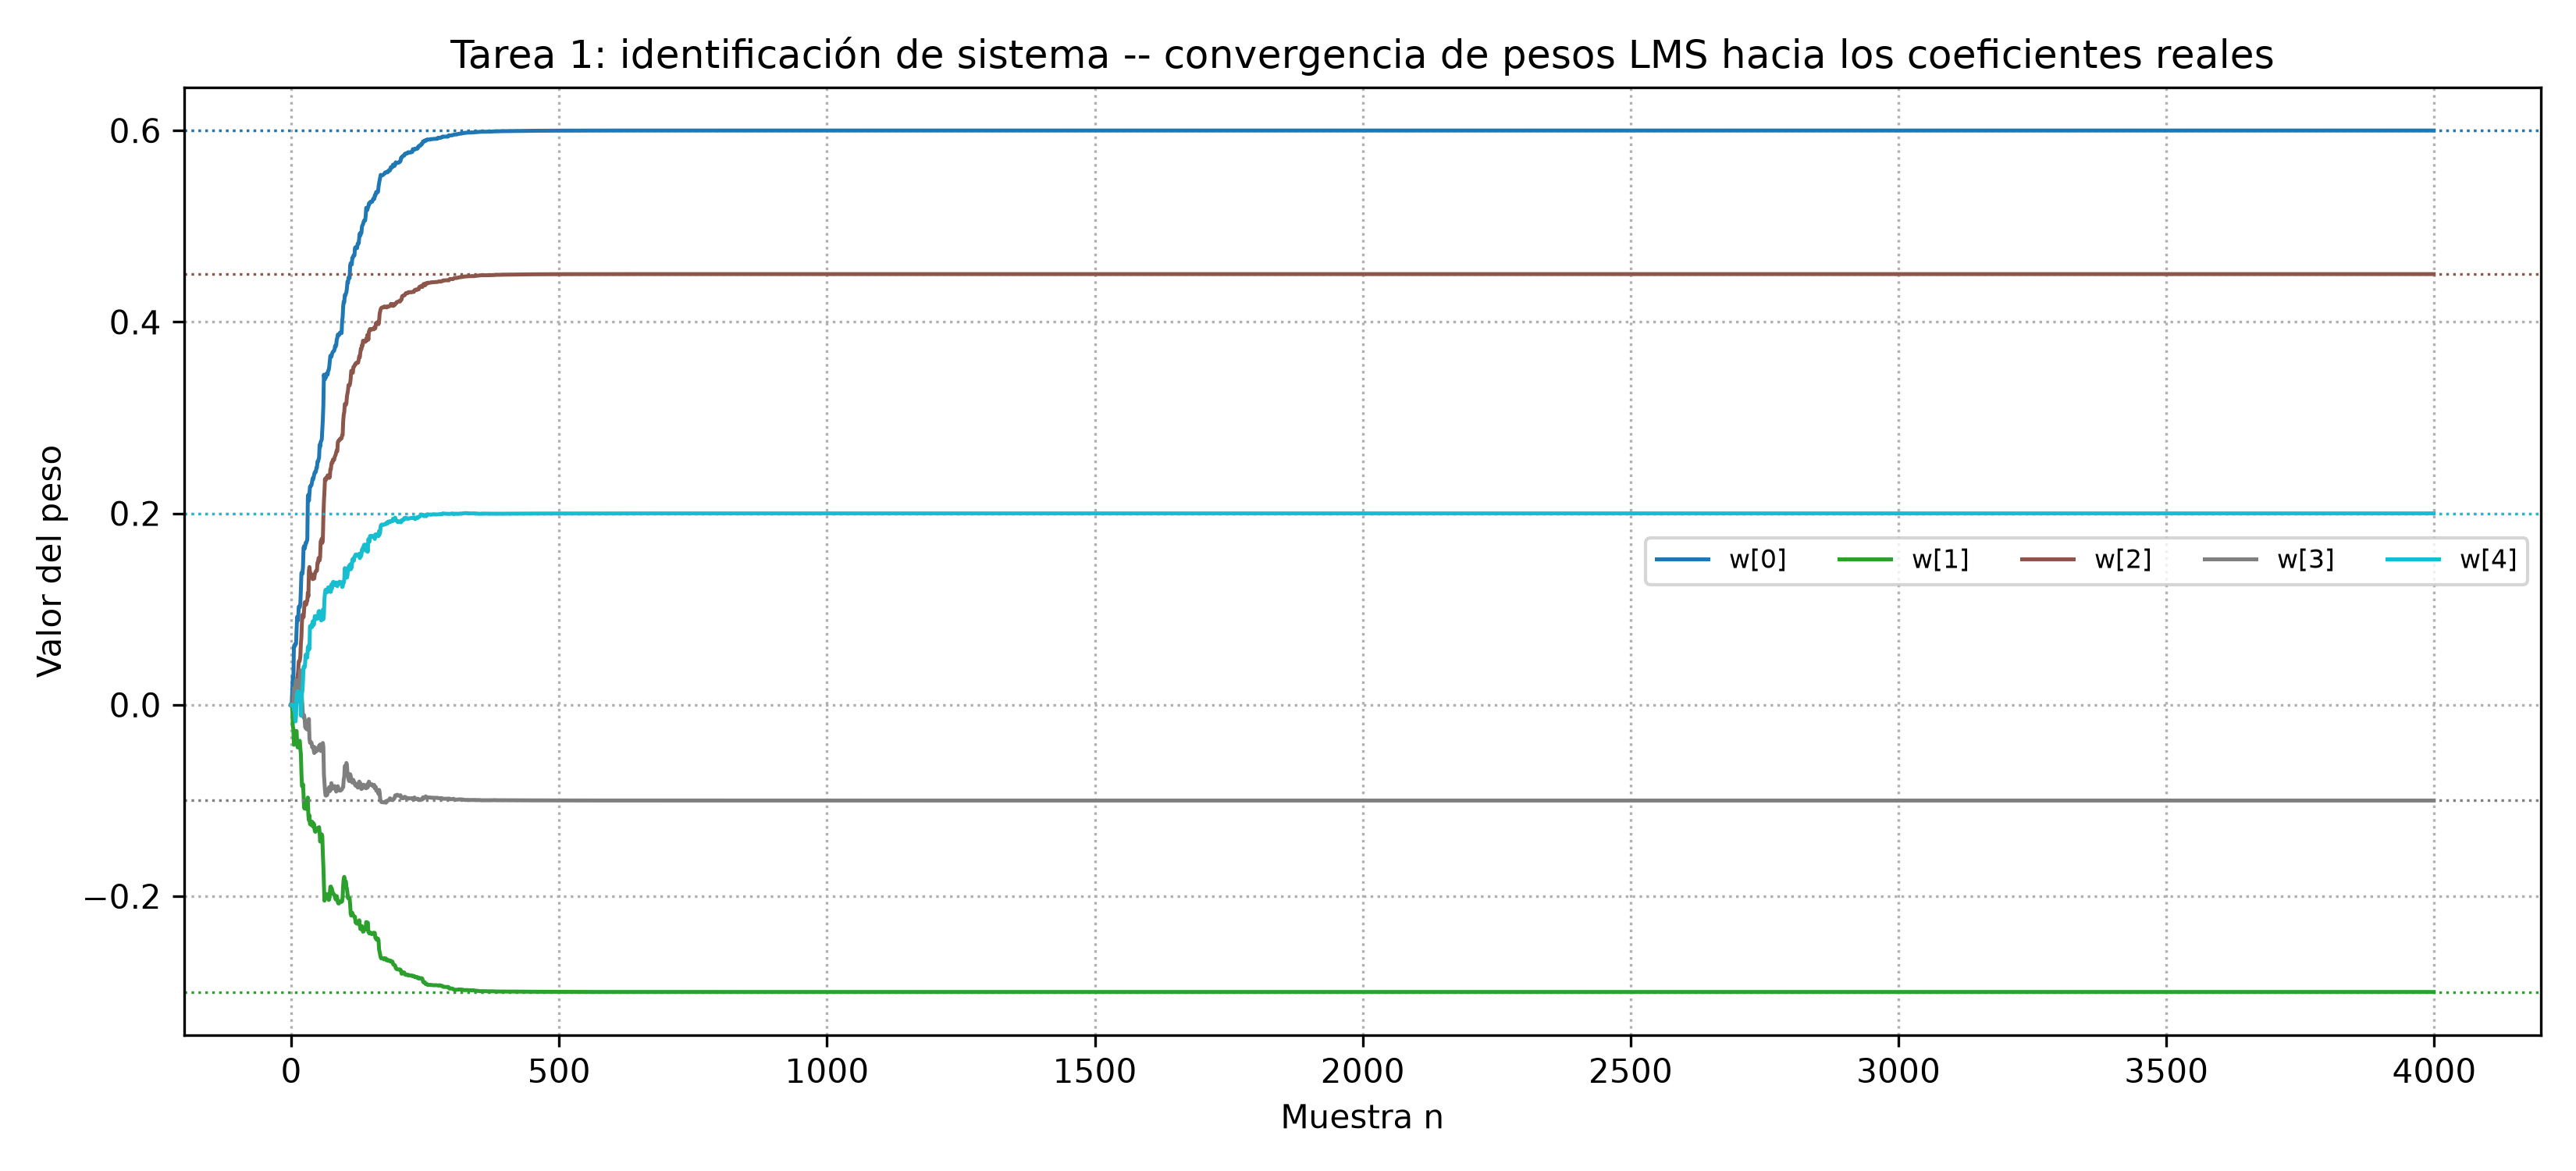
\includegraphics[width=\columnwidth]{work_eleven_t1_weight_convergence.png}
\caption{LMS: convergencia de los 5 pesos adaptados hacia los coeficientes reales del sistema FIR desconocido. Cada traza corresponde a un coeficiente individual, mostrando una convergencia monótona sin oscilación residual apreciable.}
\label{fig:work_eleven_t1_w}
\end{figure}

\begin{figure}[!t]
\centering
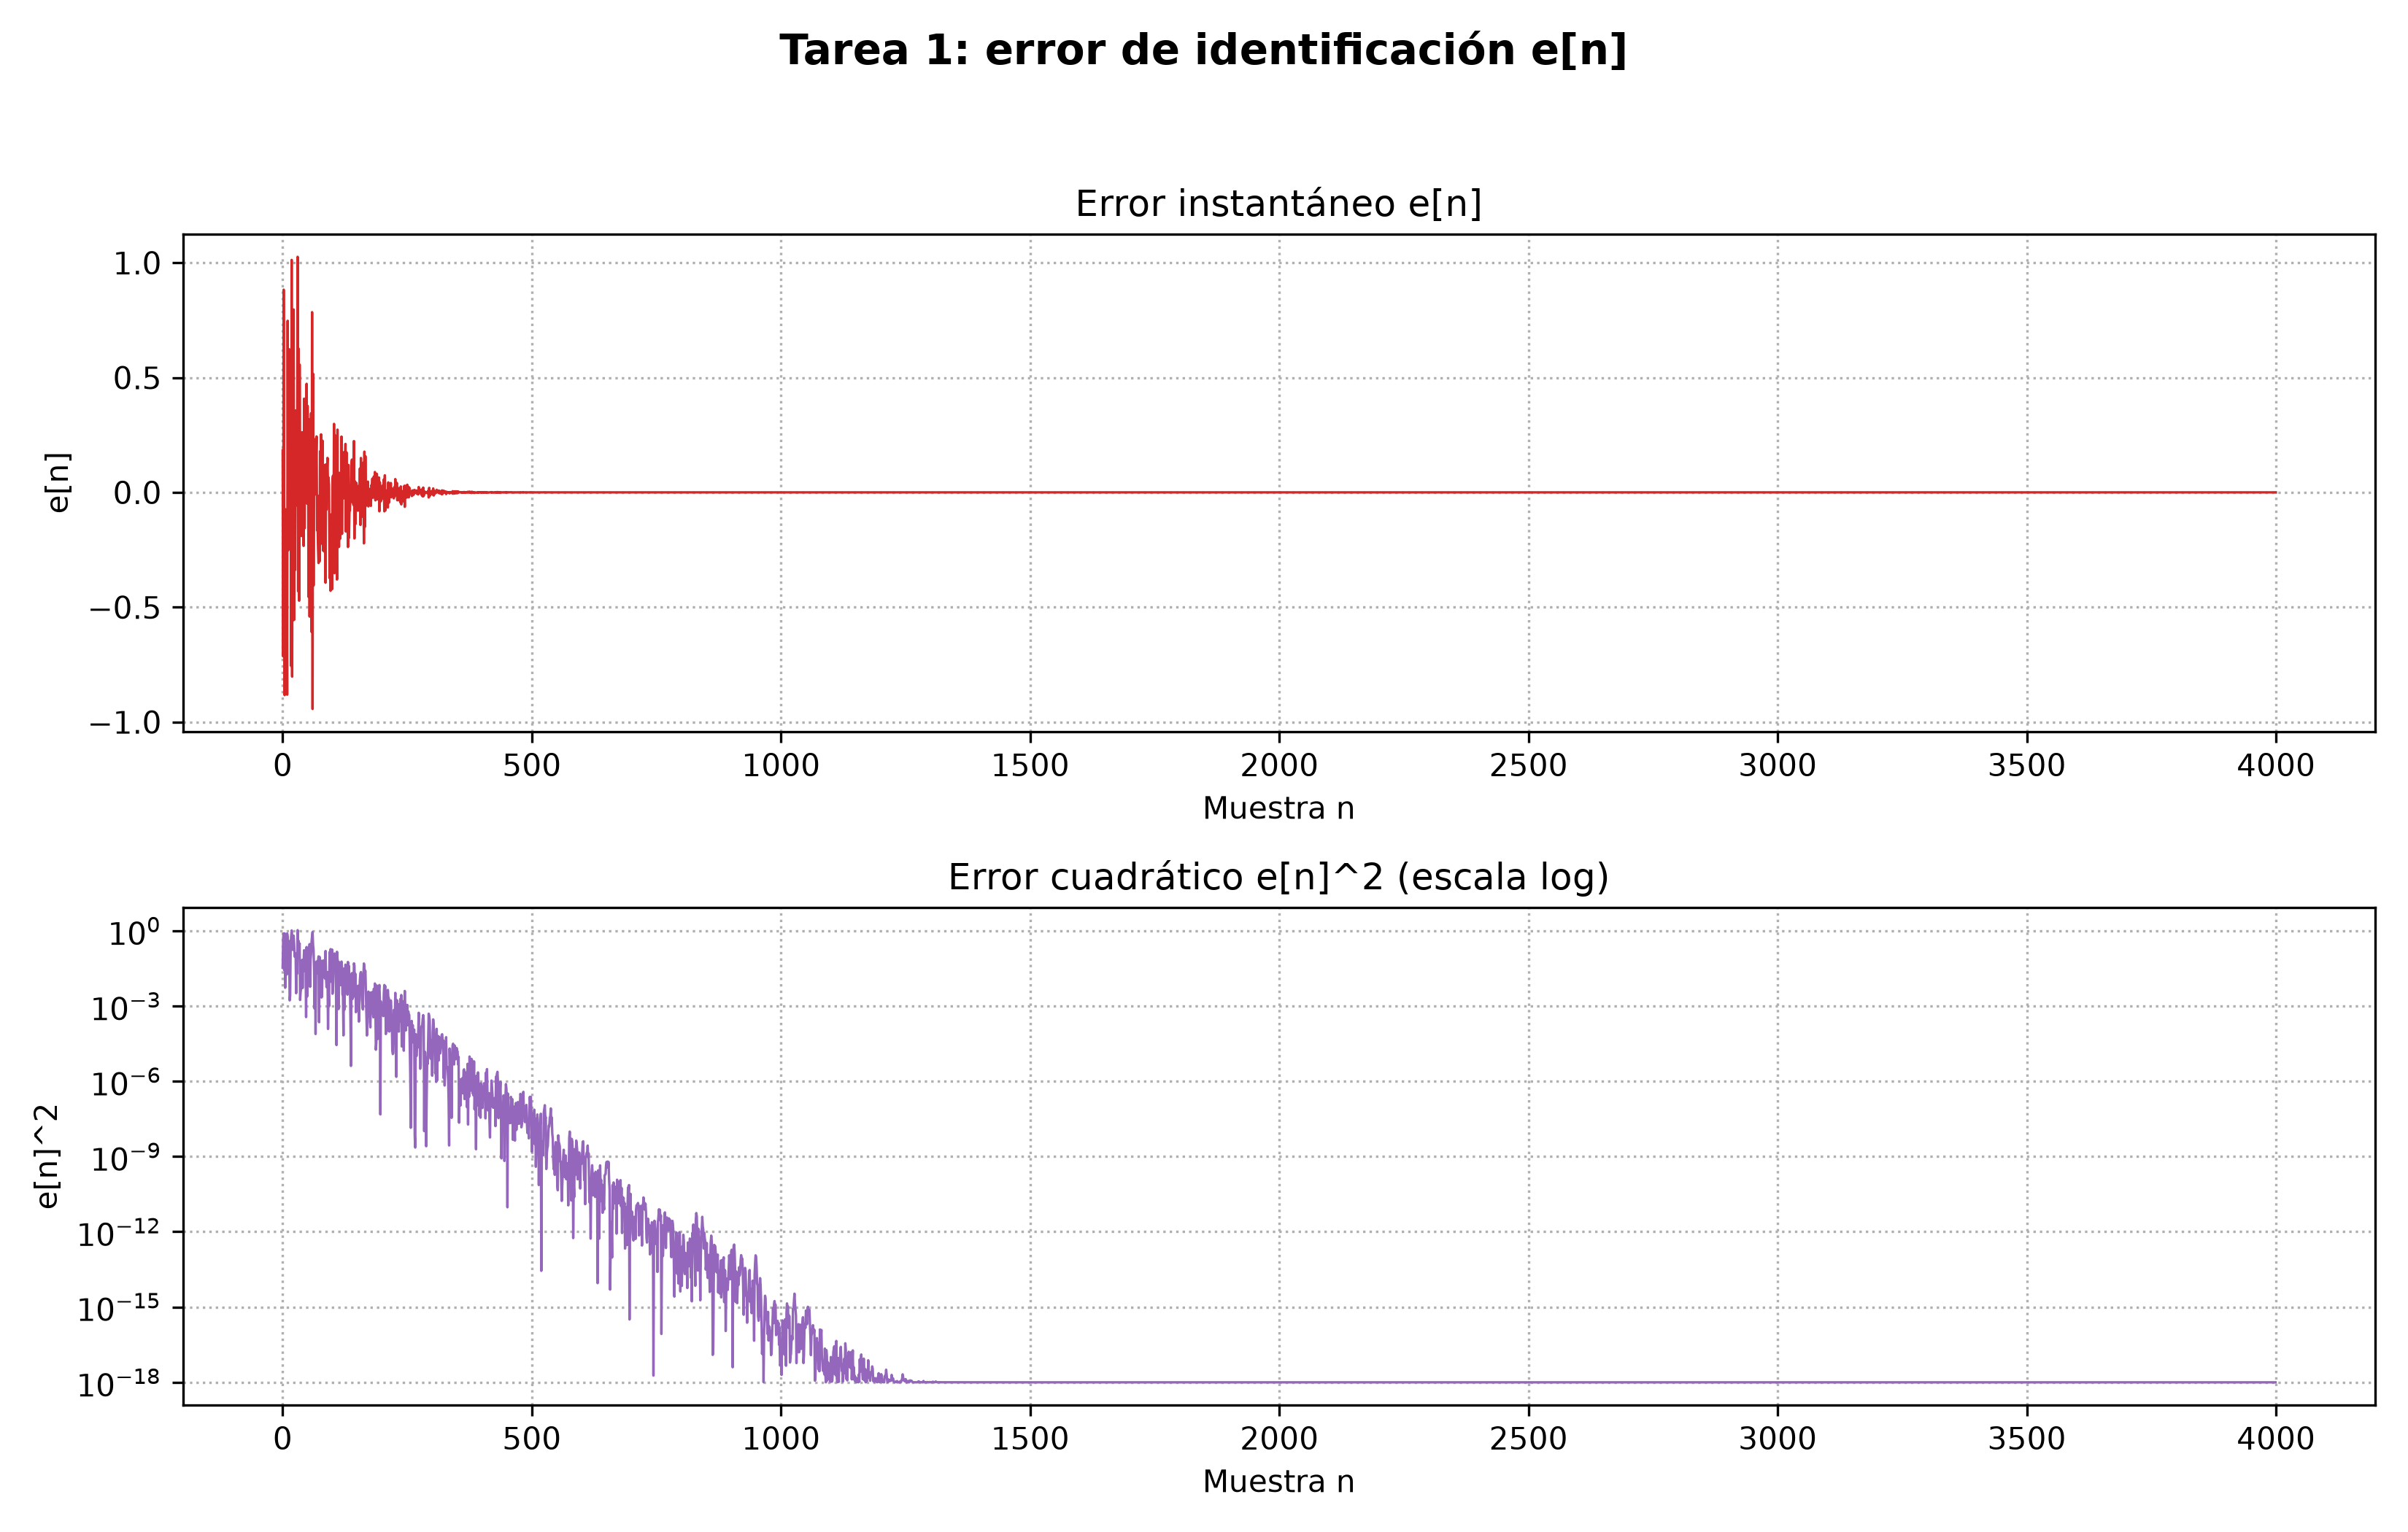
\includegraphics[width=\columnwidth]{work_eleven_t1_identification_error.png}
\caption{LMS: norma del error de identificación $\lVert w[n] - w_{\text{real}} \rVert$ en función de la iteración, en escala que evidencia el decaimiento exponencial característico del descenso de gradiente estocástico.}
\label{fig:work_eleven_t1_e}
\end{figure}

\subsubsection{Cancelación adaptativa de ruido}

El segundo experimento implementa un esquema clásico de cancelación
adaptativa de ruido (\textit{Adaptive Noise Cancellation}, ANC) de dos
entradas: una señal primaria, que contiene la señal de interés
contaminada por ruido, y una señal de referencia correlacionada con ese
ruido pero sin contenido de la señal de interés —la configuración
típica cuando se dispone de un sensor adicional capaz de captar
predominantemente la fuente de ruido. El filtro LMS usa la referencia
de ruido como entrada $x[n]$ y la señal primaria contaminada como señal
deseada $d[n]$; a medida que converge, la salida del filtro $y[n]$ se
aproxima a la componente de ruido presente en la señal primaria, de
modo que el error $e[n] = d[n] - y[n]$ —que es la salida real de
interés del sistema, no un subproducto a minimizar— tiende hacia la
señal limpia original.

Se aplicó este esquema sobre dos señales de naturaleza distinta para
evaluar su robustez: un tono sintético de 60~Hz, elegido por
consistencia con el resto de esta serie de trabajos, y una grabación de
audio real (el mismo archivo \texttt{gato.ogg} usado en trabajos
anteriores de este repositorio, copiado localmente para mantener esta
carpeta autocontenida). En el caso del tono, la desviación estándar del
residuo —la medida de cuánto ruido queda tras el filtrado— cayó de
0.617 antes del filtrado a 0.135 después, una reducción de ruido de
aproximadamente 4.6 veces en términos de desviación estándar (y por lo
tanto, de más de 20 veces en potencia). El comportamiento sobre el
audio real (Fig.~\ref{fig:work_eleven_t2b}) confirma que el algoritmo
no depende de propiedades idealizadas de una señal sintética y
generaliza correctamente a una señal con contenido espectral más rico
y no estacionario.

\begin{figure}[!t]
\centering
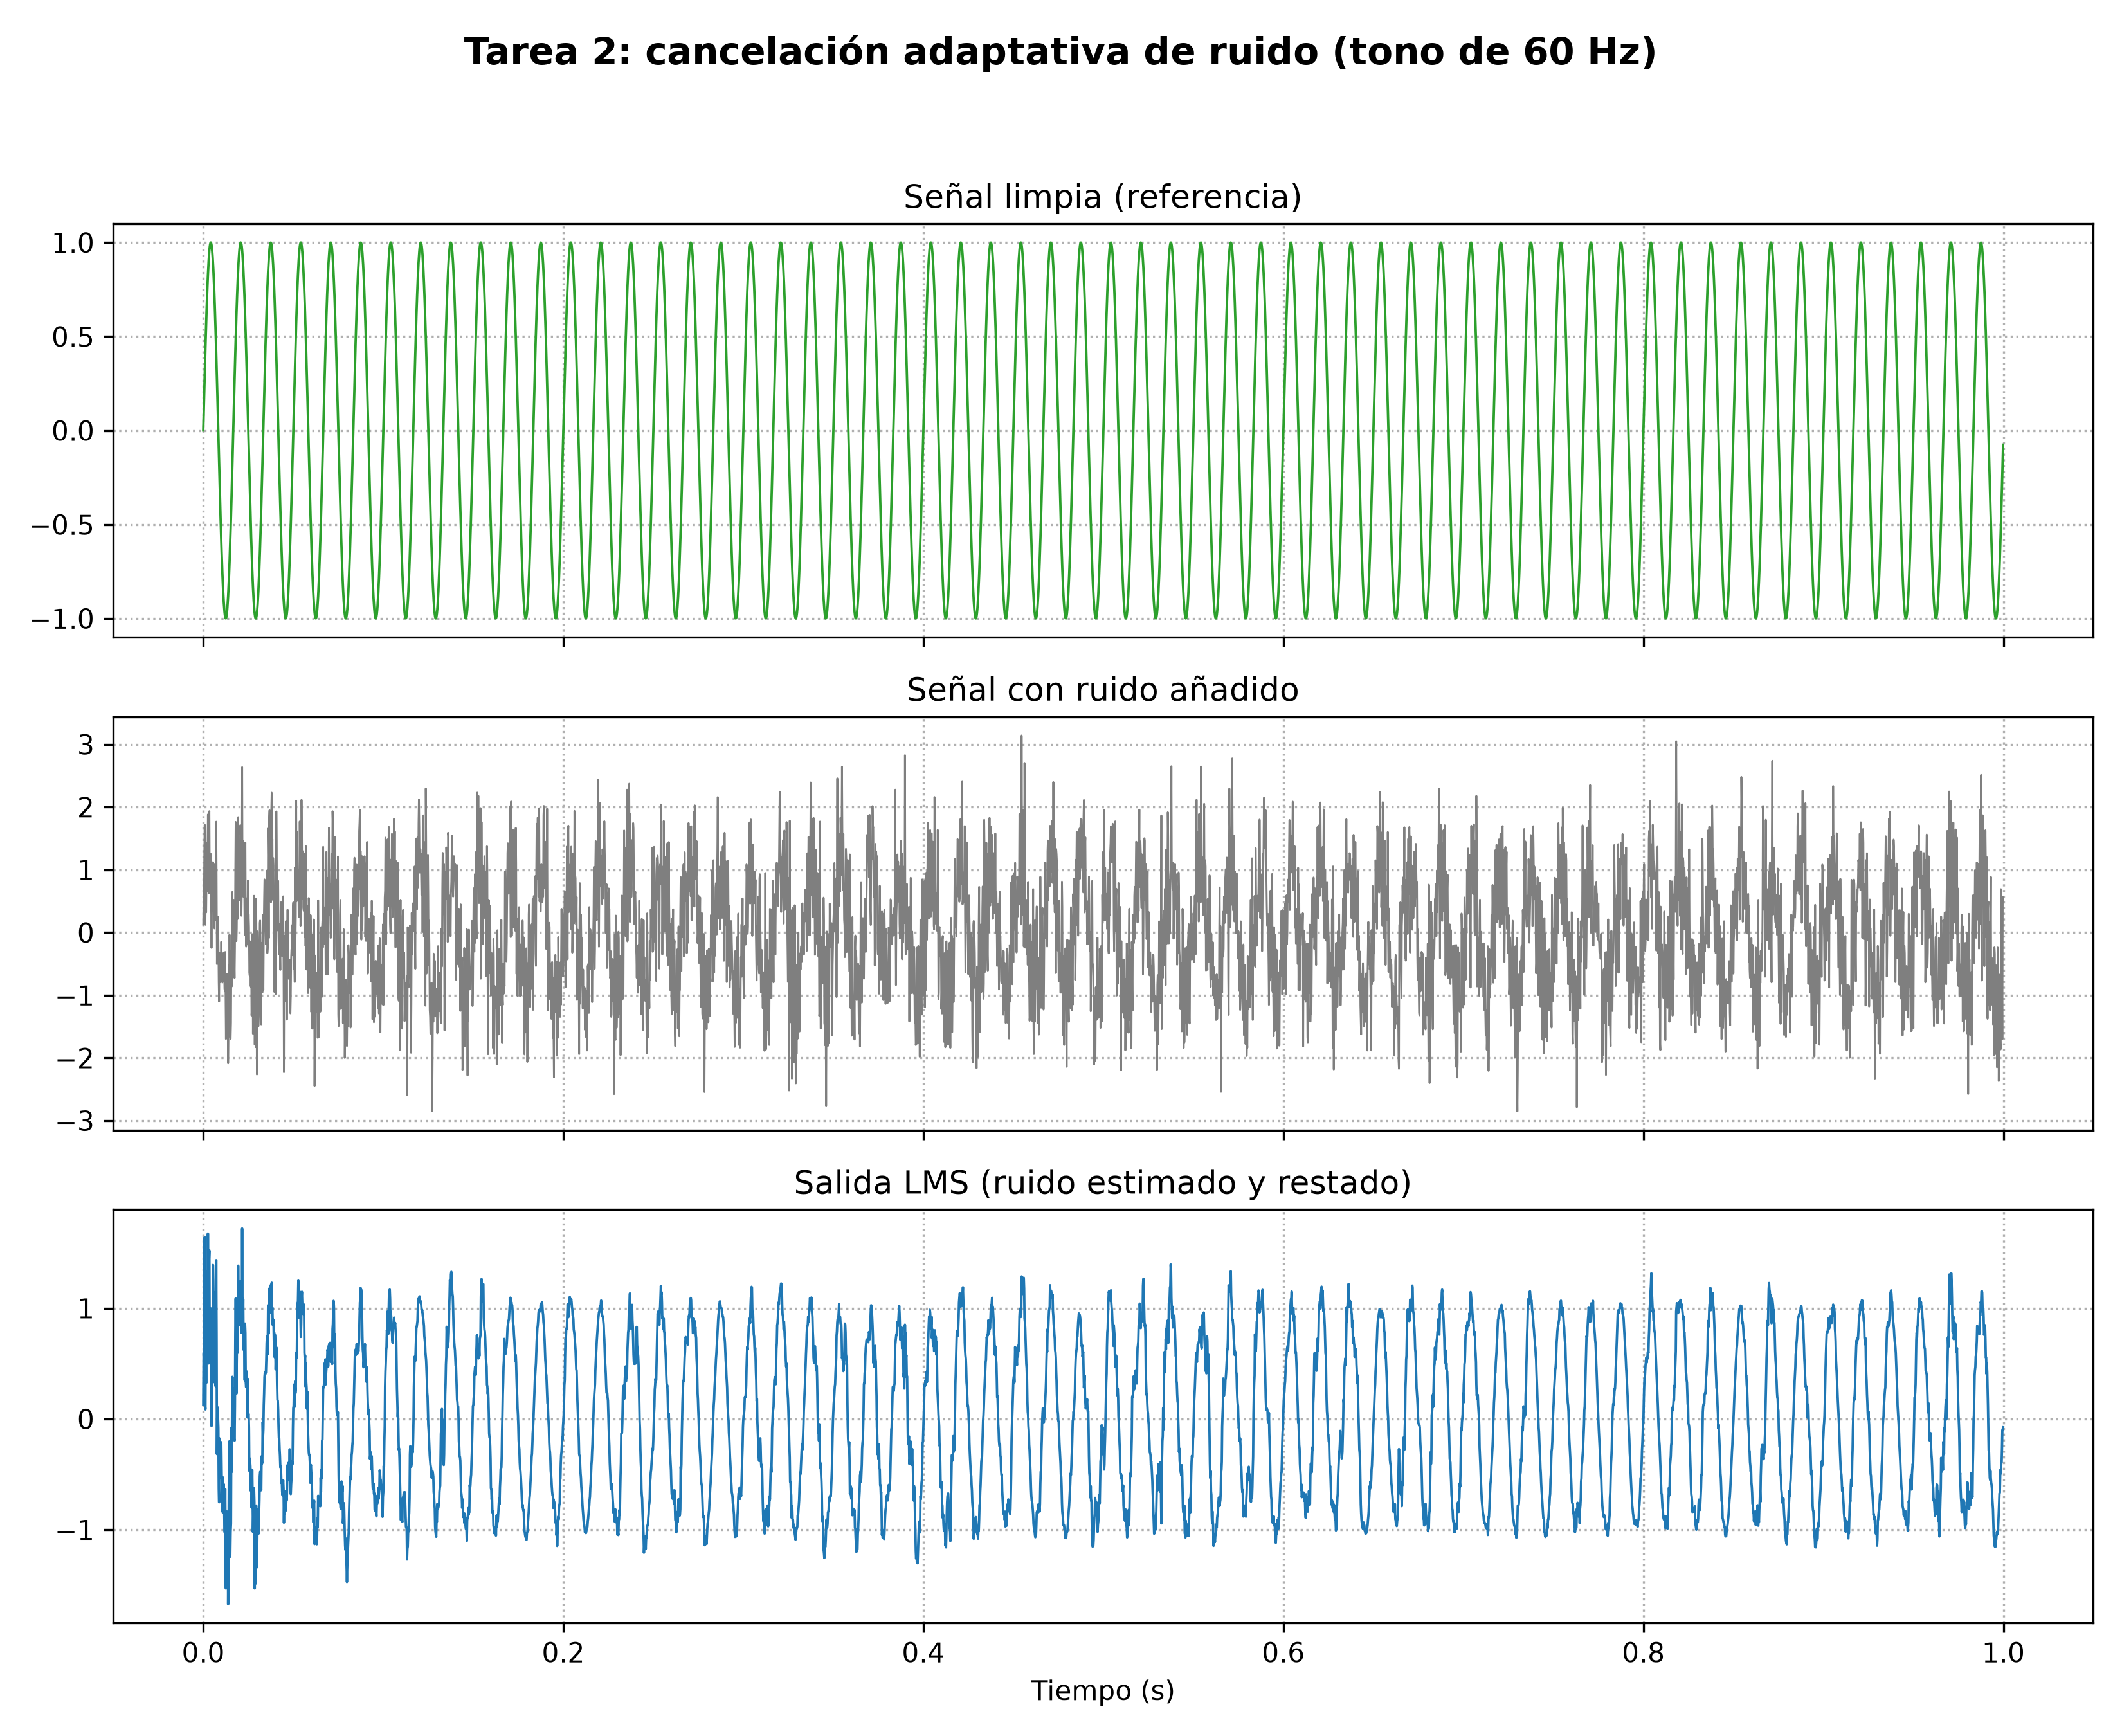
\includegraphics[width=\columnwidth]{work_eleven_t2_noise_cancellation_tone.png}
\caption{LMS: cancelación adaptativa de ruido sobre un tono de 60~Hz. De arriba a abajo: señal limpia de referencia, señal primaria contaminada, señal recuperada tras la cancelación.}
\label{fig:work_eleven_t2}
\end{figure}

\begin{figure}[!t]
\centering
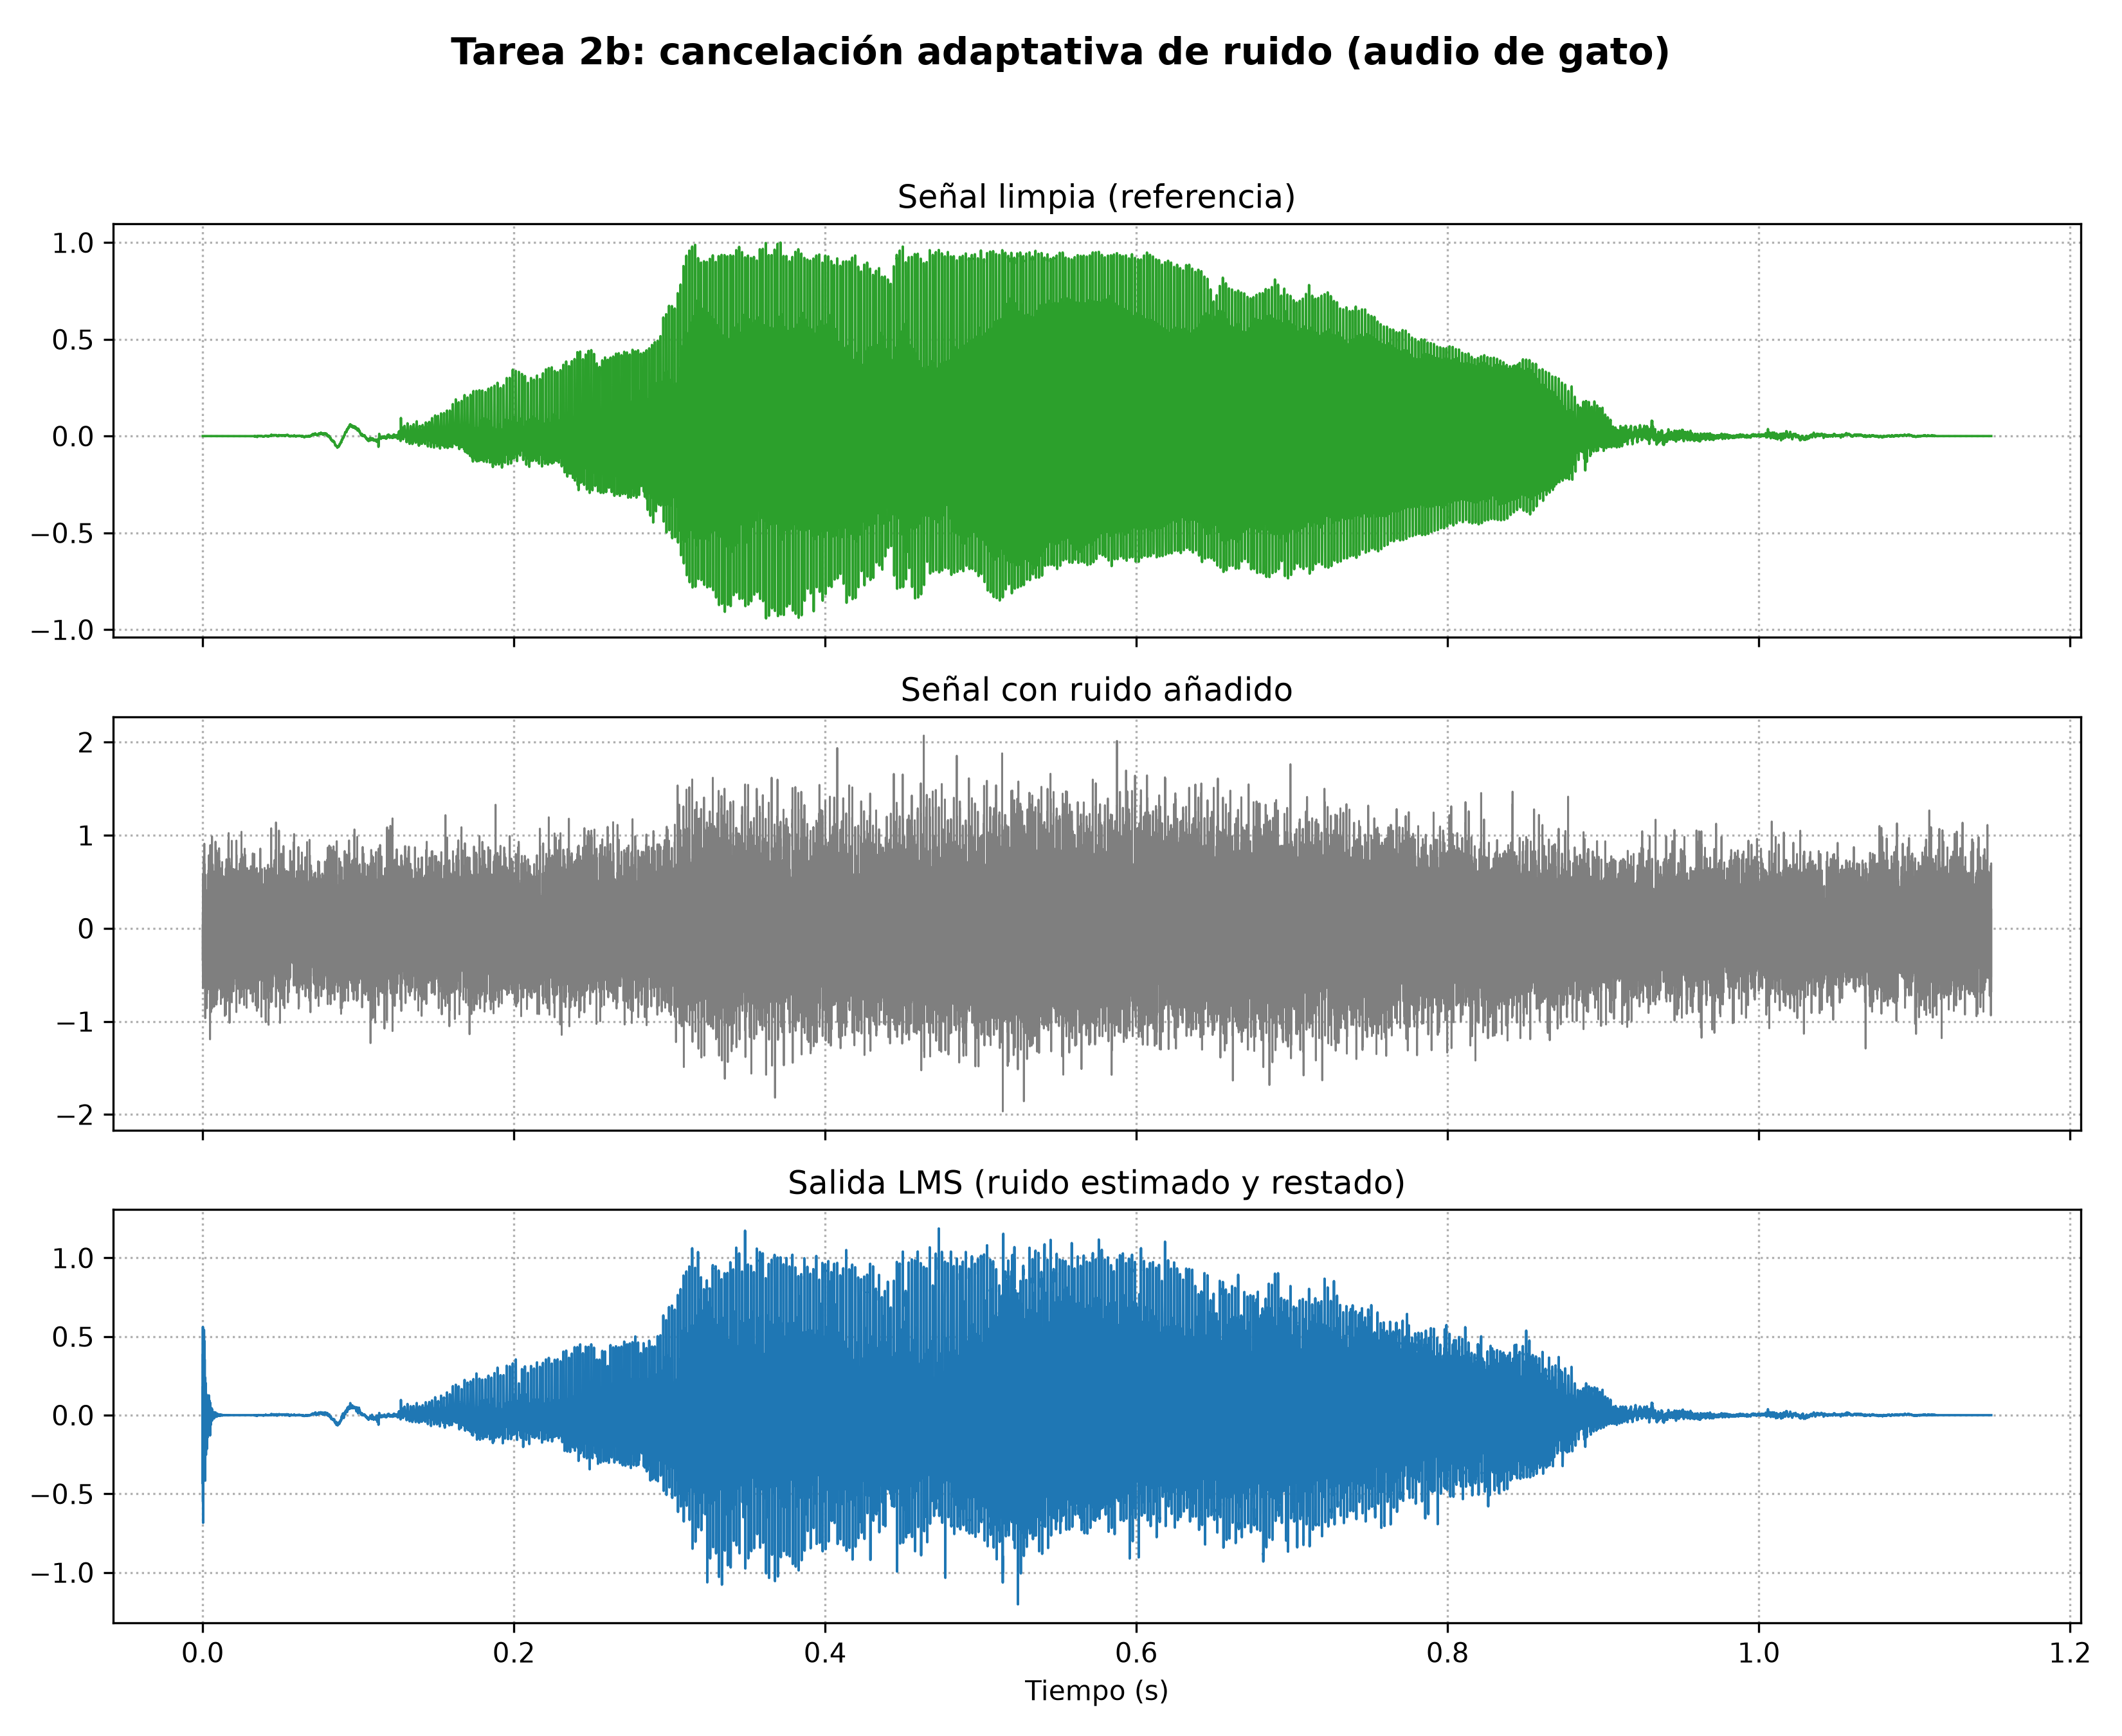
\includegraphics[width=\columnwidth]{work_eleven_t2b_noise_cancellation_cat.png}
\caption{LMS: cancelación adaptativa de ruido sobre una grabación de audio real, mostrando que el esquema de dos entradas generaliza más allá de señales sintéticas de banda angosta.}
\label{fig:work_eleven_t2b}
\end{figure}

\subsubsection{Convergencia frente al tamaño de paso $\mu$}

El tercer experimento caracteriza de forma sistemática el compromiso
velocidad/estabilidad discutido en la introducción, barriendo el mismo
problema de identificación de sistema sobre un conjunto de valores de
$\mu$ que abarca varios órdenes de magnitud
(Fig.~\ref{fig:work_eleven_t3}). Con $\mu = 0.001$, la convergencia es
notablemente lenta y, dentro del número de iteraciones ejecutado, queda
un error residual medible: el filtro todavía está en camino hacia la
solución óptima, no la ha alcanzado. Con $\mu$ en el rango de 0.01 a
0.1, la convergencia es rápida y el filtro alcanza un error
prácticamente nulo (limitado únicamente por la precisión numérica de
punto flotante), sin señales de oscilación o inestabilidad. Con
$\mu = 0.5$, en cambio, el filtro diverge de forma manifiesta,
acumulando error hasta desbordar numéricamente (de ahí la advertencia
de \textit{overflow} de NumPy registrada intencionalmente durante la
ejecución de pruebas, que documenta precisamente este comportamiento
esperado).

Este resultado experimental se corresponde de forma precisa con la
cota teórica de estabilidad de LMS, que establece que el algoritmo
converge en media cuadrática si y solo si
\begin{equation}
0 < \mu < \frac{2}{\lambda_{\max}},
\end{equation}
donde $\lambda_{\max}$ es el mayor autovalor de la matriz de
autocorrelación $R = E[x[n]\,x[n]^\top]$ de la entrada. Para una
entrada de ruido blanco con $N$ coeficientes y varianza $\sigma_x^2$,
la matriz de autocorrelación es aproximadamente $\sigma_x^2 I$, de modo
que todos sus autovalores son iguales a $\sigma_x^2$ y la cota se
simplifica a $\mu < 2/(N\sigma_x^2)$. Para la configuración usada en
este laboratorio ($N=5$ coeficientes, $\sigma_x^2 \approx 1$), esta
cota resulta en $\mu \lesssim 0.4$, consistente con la estabilidad
observada en $\mu \leq 0.1$ y la divergencia observada en $\mu = 0.5$,
que queda justo por encima del límite teórico.

\begin{figure}[!t]
\centering
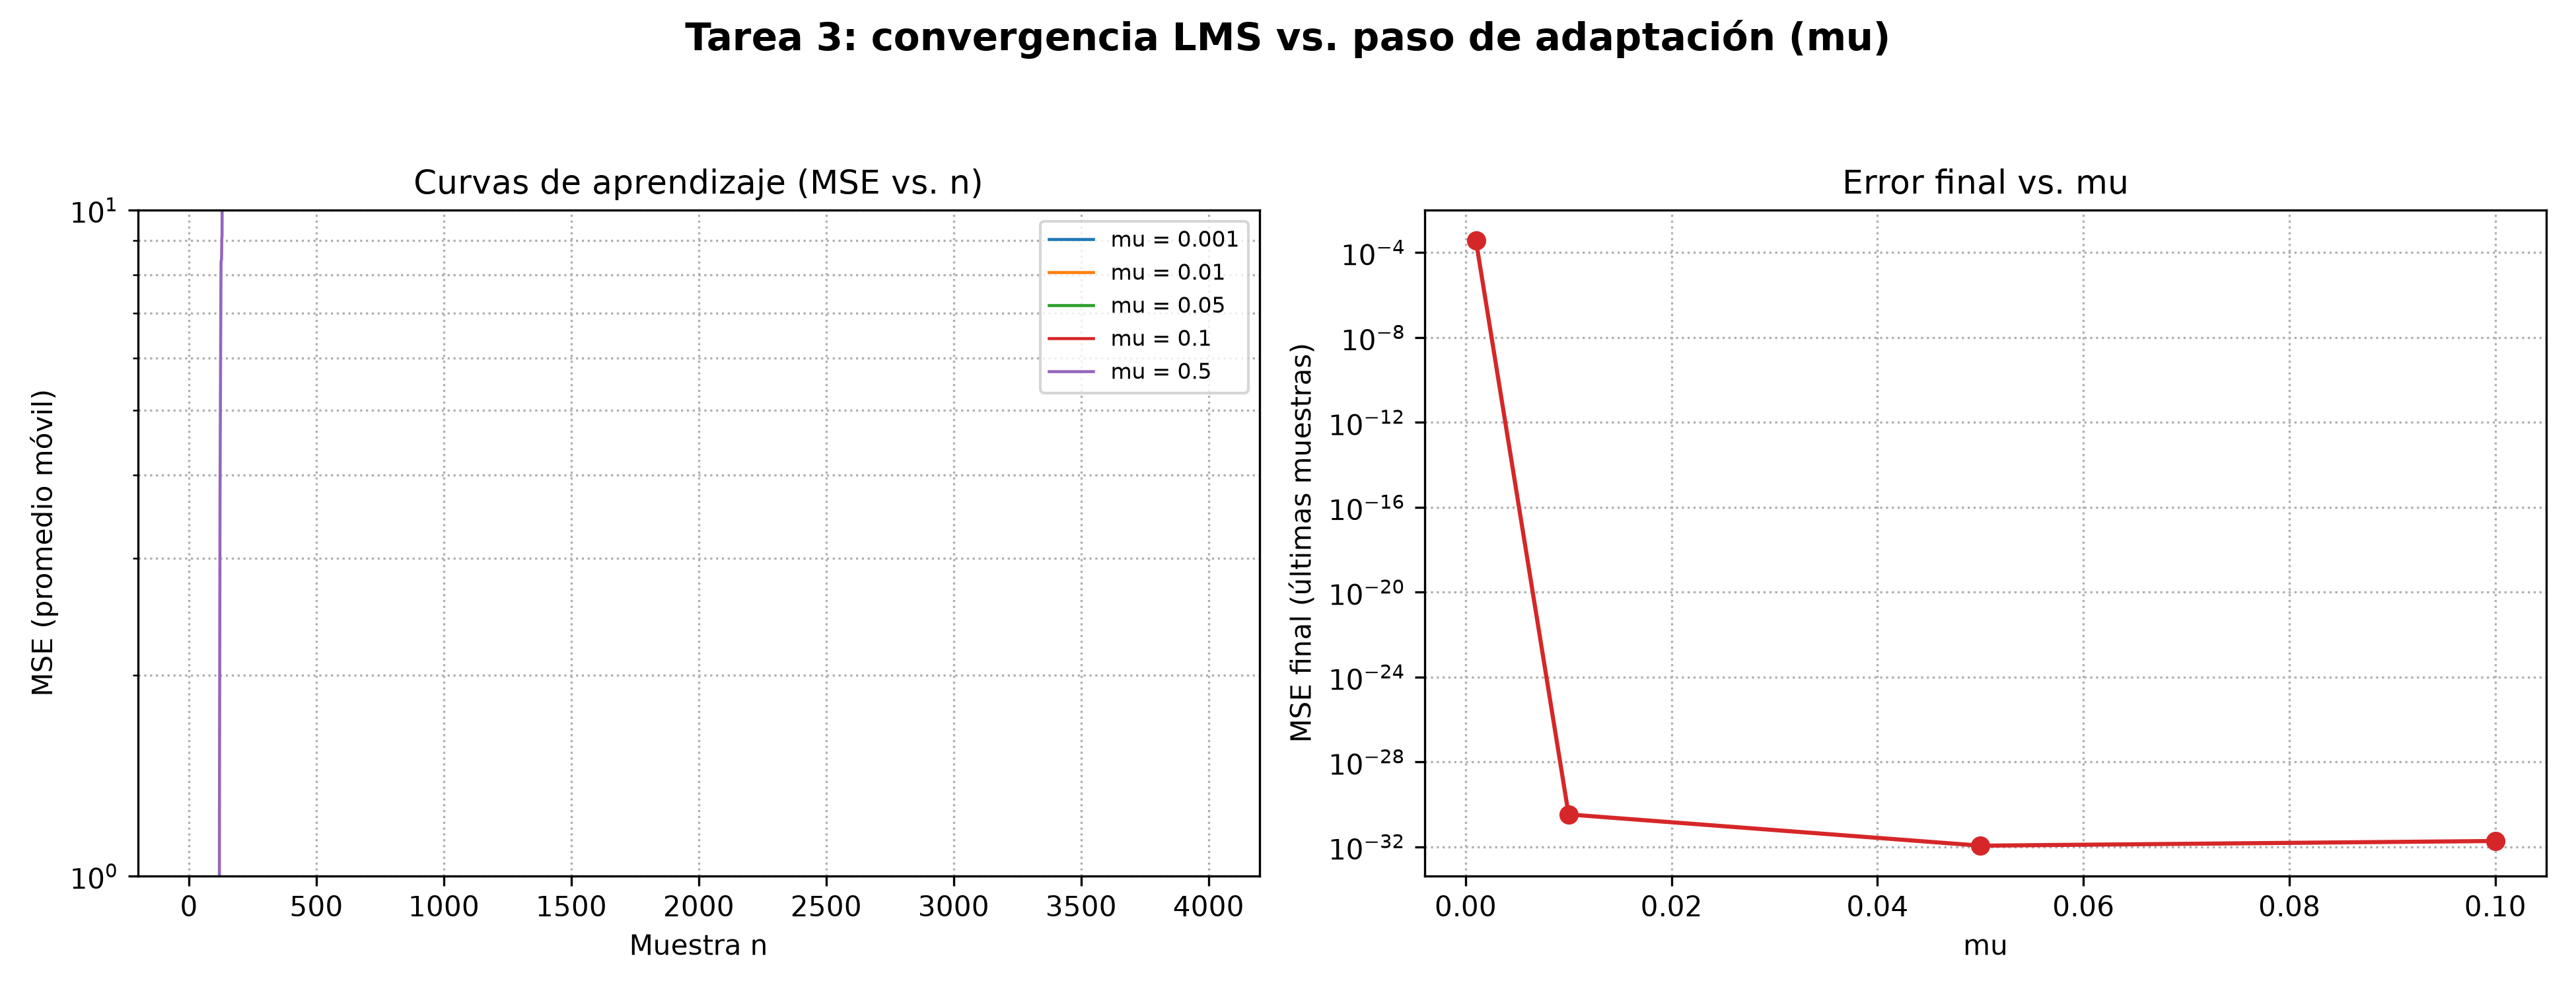
\includegraphics[width=\columnwidth]{work_eleven_t3_mu_sweep.png}
\caption{LMS: error cuadrático medio en estado estacionario en función de $\mu$ (escala logarítmica), evidenciando las tres regiones de comportamiento: convergencia lenta ($\mu$ pequeño), convergencia rápida y estable (región intermedia), y divergencia ($\mu$ por encima de la cota teórica $2/\lambda_{\max}$).}
\label{fig:work_eleven_t3}
\end{figure}

% ============================================================
% WORK_TWELVE: Filtro adaptativo NLMS, comparacion contra LMS
% ============================================================

\subsection{WORK\_TWELVE: Filtro adaptativo NLMS}

Se implementó NLMS (Ec.~\ref{eq:nlms}) desde cero en
\texttt{nlms\_lab/adaptive.py}, de forma completamente independiente a
WORK\_ELEVEN —ninguno de los dos trabajos importa código del otro,
cada uno reimplementa localmente lo que necesita—, y se evaluó sobre
los mismos tres tipos de experimento usados para LMS, añadiendo además
una comparación directa entre ambos algoritmos bajo condiciones de
potencia de entrada no estacionaria.

\subsubsection{Identificación de sistema}

Sobre el mismo tipo de problema de identificación ciega de un filtro
FIR de 5 coeficientes excitado con ruido blanco descrito en la sección
anterior, NLMS partió de un error inicial de pesos de 0.9354 —el error
correspondiente a inicializar el vector de pesos en cero antes de
cualquier adaptación— y convergió a un error final prácticamente nulo
($\approx 10^{-6}$, Fig.~\ref{fig:work_twelve_t1}). La velocidad de
convergencia observada es comparable a la mejor región de LMS
(Sección~\ref{sec:resultados}, barrido de $\mu$), lo cual es esperable:
cuando la potencia de la señal de entrada es constante, el paso
efectivo de NLMS se estabiliza en un valor fijo y el algoritmo se
comporta de manera muy similar a LMS con un $\mu$ bien ajustado para
esa potencia particular. La diferencia entre ambos algoritmos solo se
hace evidente —y relevante en la práctica— cuando esa potencia deja de
ser constante, como se explora en la Sección~\ref{sec:nlms_vs_lms}.

\begin{figure}[!t]
\centering
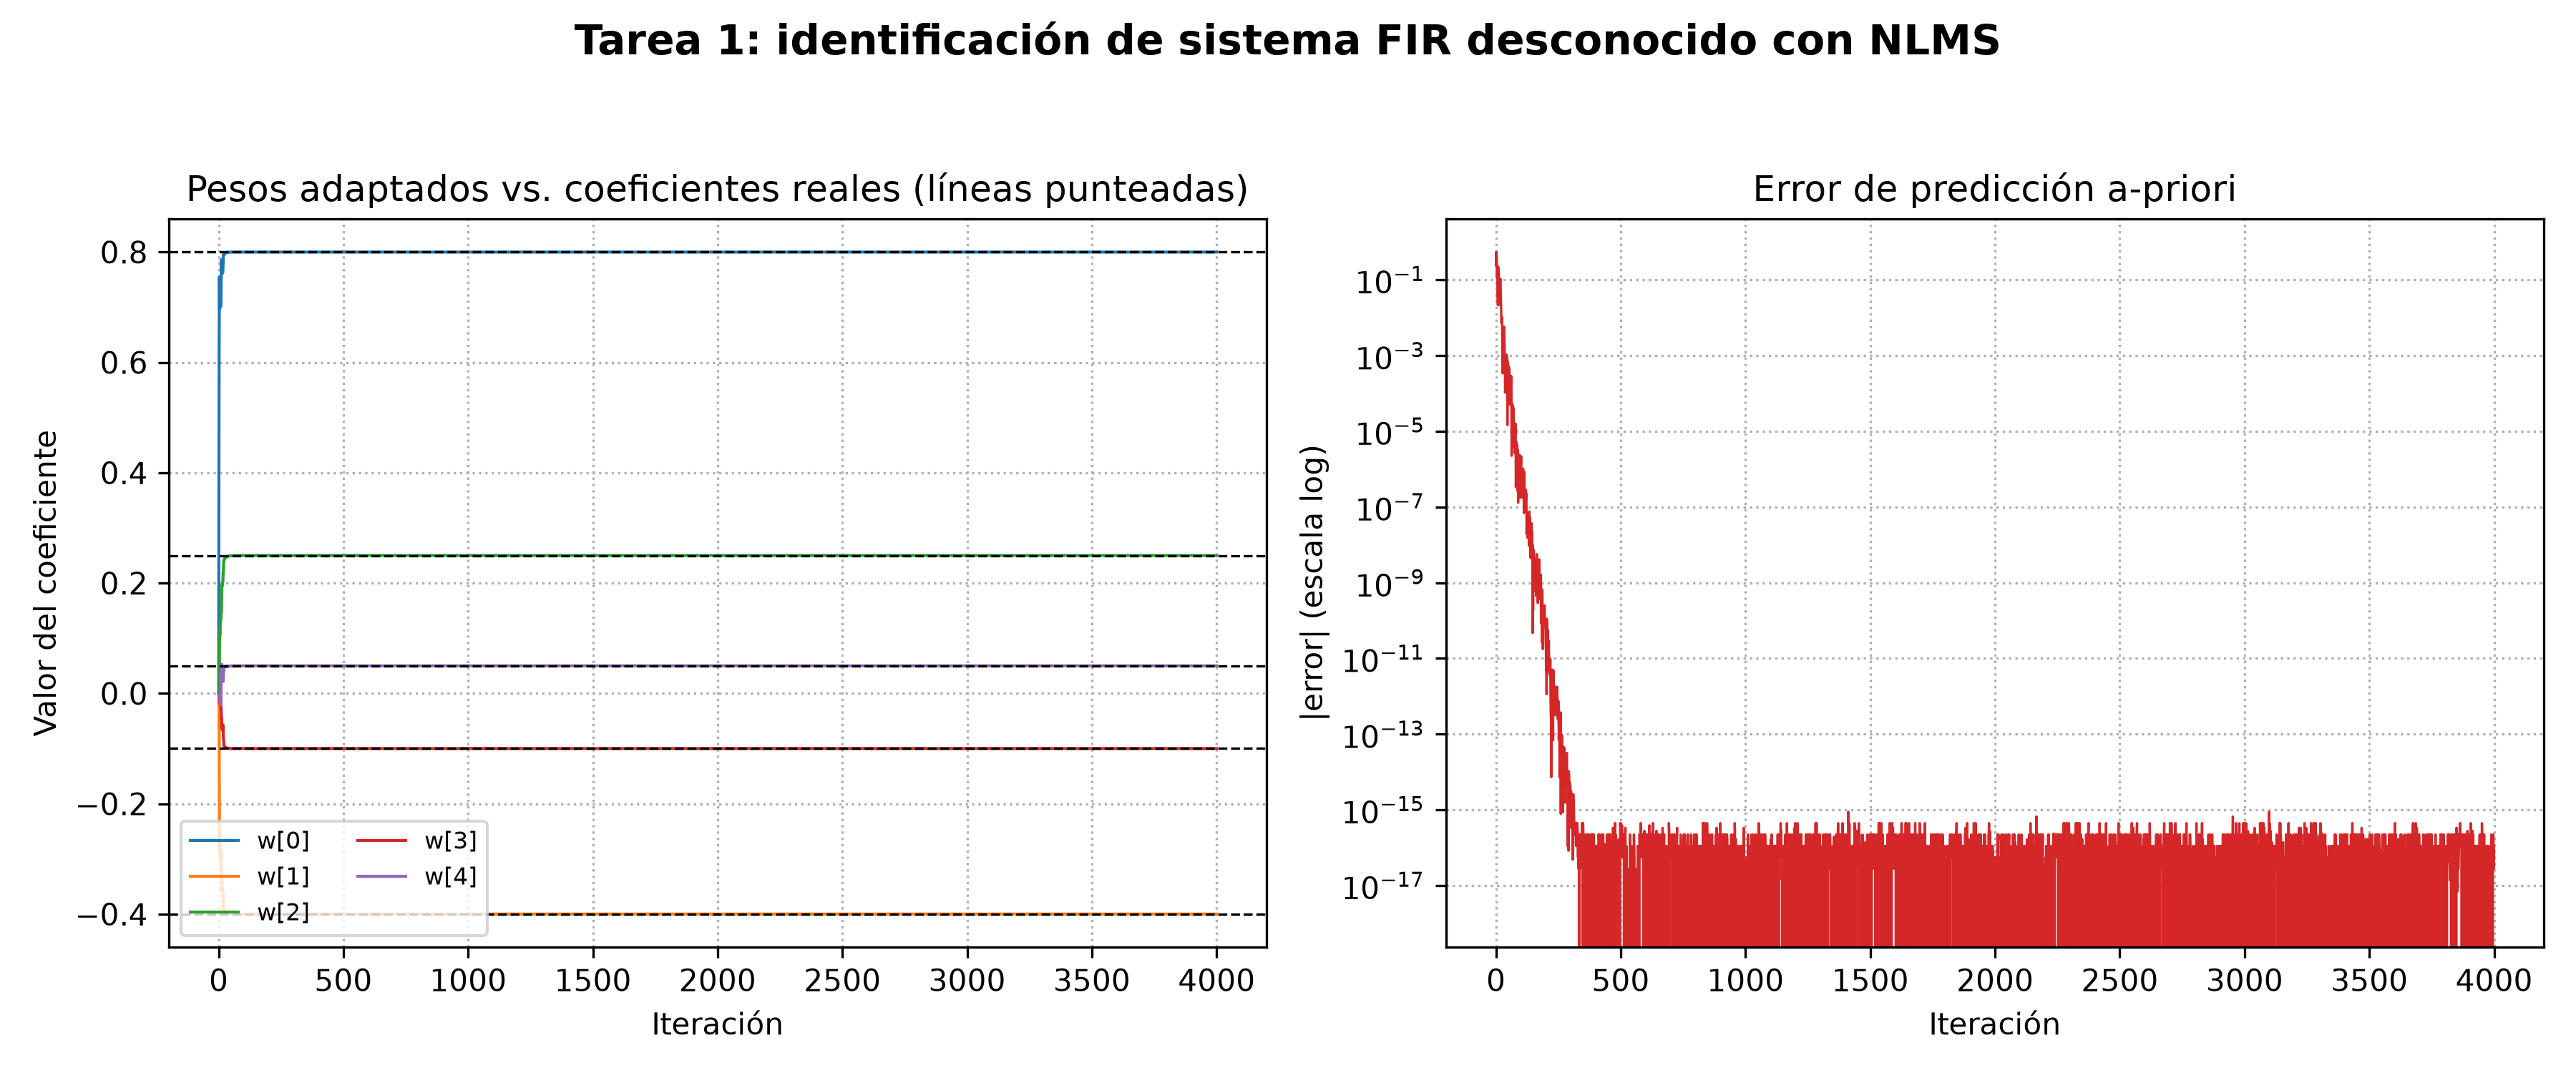
\includegraphics[width=\columnwidth]{work_twelve_t1_system_identification.png}
\caption{NLMS: convergencia de los pesos del filtro hacia los coeficientes reales del sistema FIR desconocido (panel superior) y evolución del error de identificación (panel inferior).}
\label{fig:work_twelve_t1}
\end{figure}

\subsubsection{Cancelación adaptativa de ruido}

Usando el mismo esquema de cancelación de ruido de dos entradas
descrito para LMS, NLMS recuperó tanto un tono sintético de 60~Hz como
la grabación de audio real contaminados con ruido correlacionado con
una señal de referencia. En el caso del tono, la desviación estándar
del residuo cayó de 0.5036 antes del filtrado a 0.1614 después —una
reducción de aproximadamente 3.1 veces en desviación estándar, del
mismo orden de magnitud que la obtenida con LMS bajo condiciones de
potencia constante, lo cual es consistente con la expectativa teórica
de que ambos algoritmos deberían comportarse de forma comparable
cuando no hay variación de potencia que explotar
(Fig.~\ref{fig:work_twelve_t2a}, \ref{fig:work_twelve_t2b}).

\begin{figure}[!t]
\centering
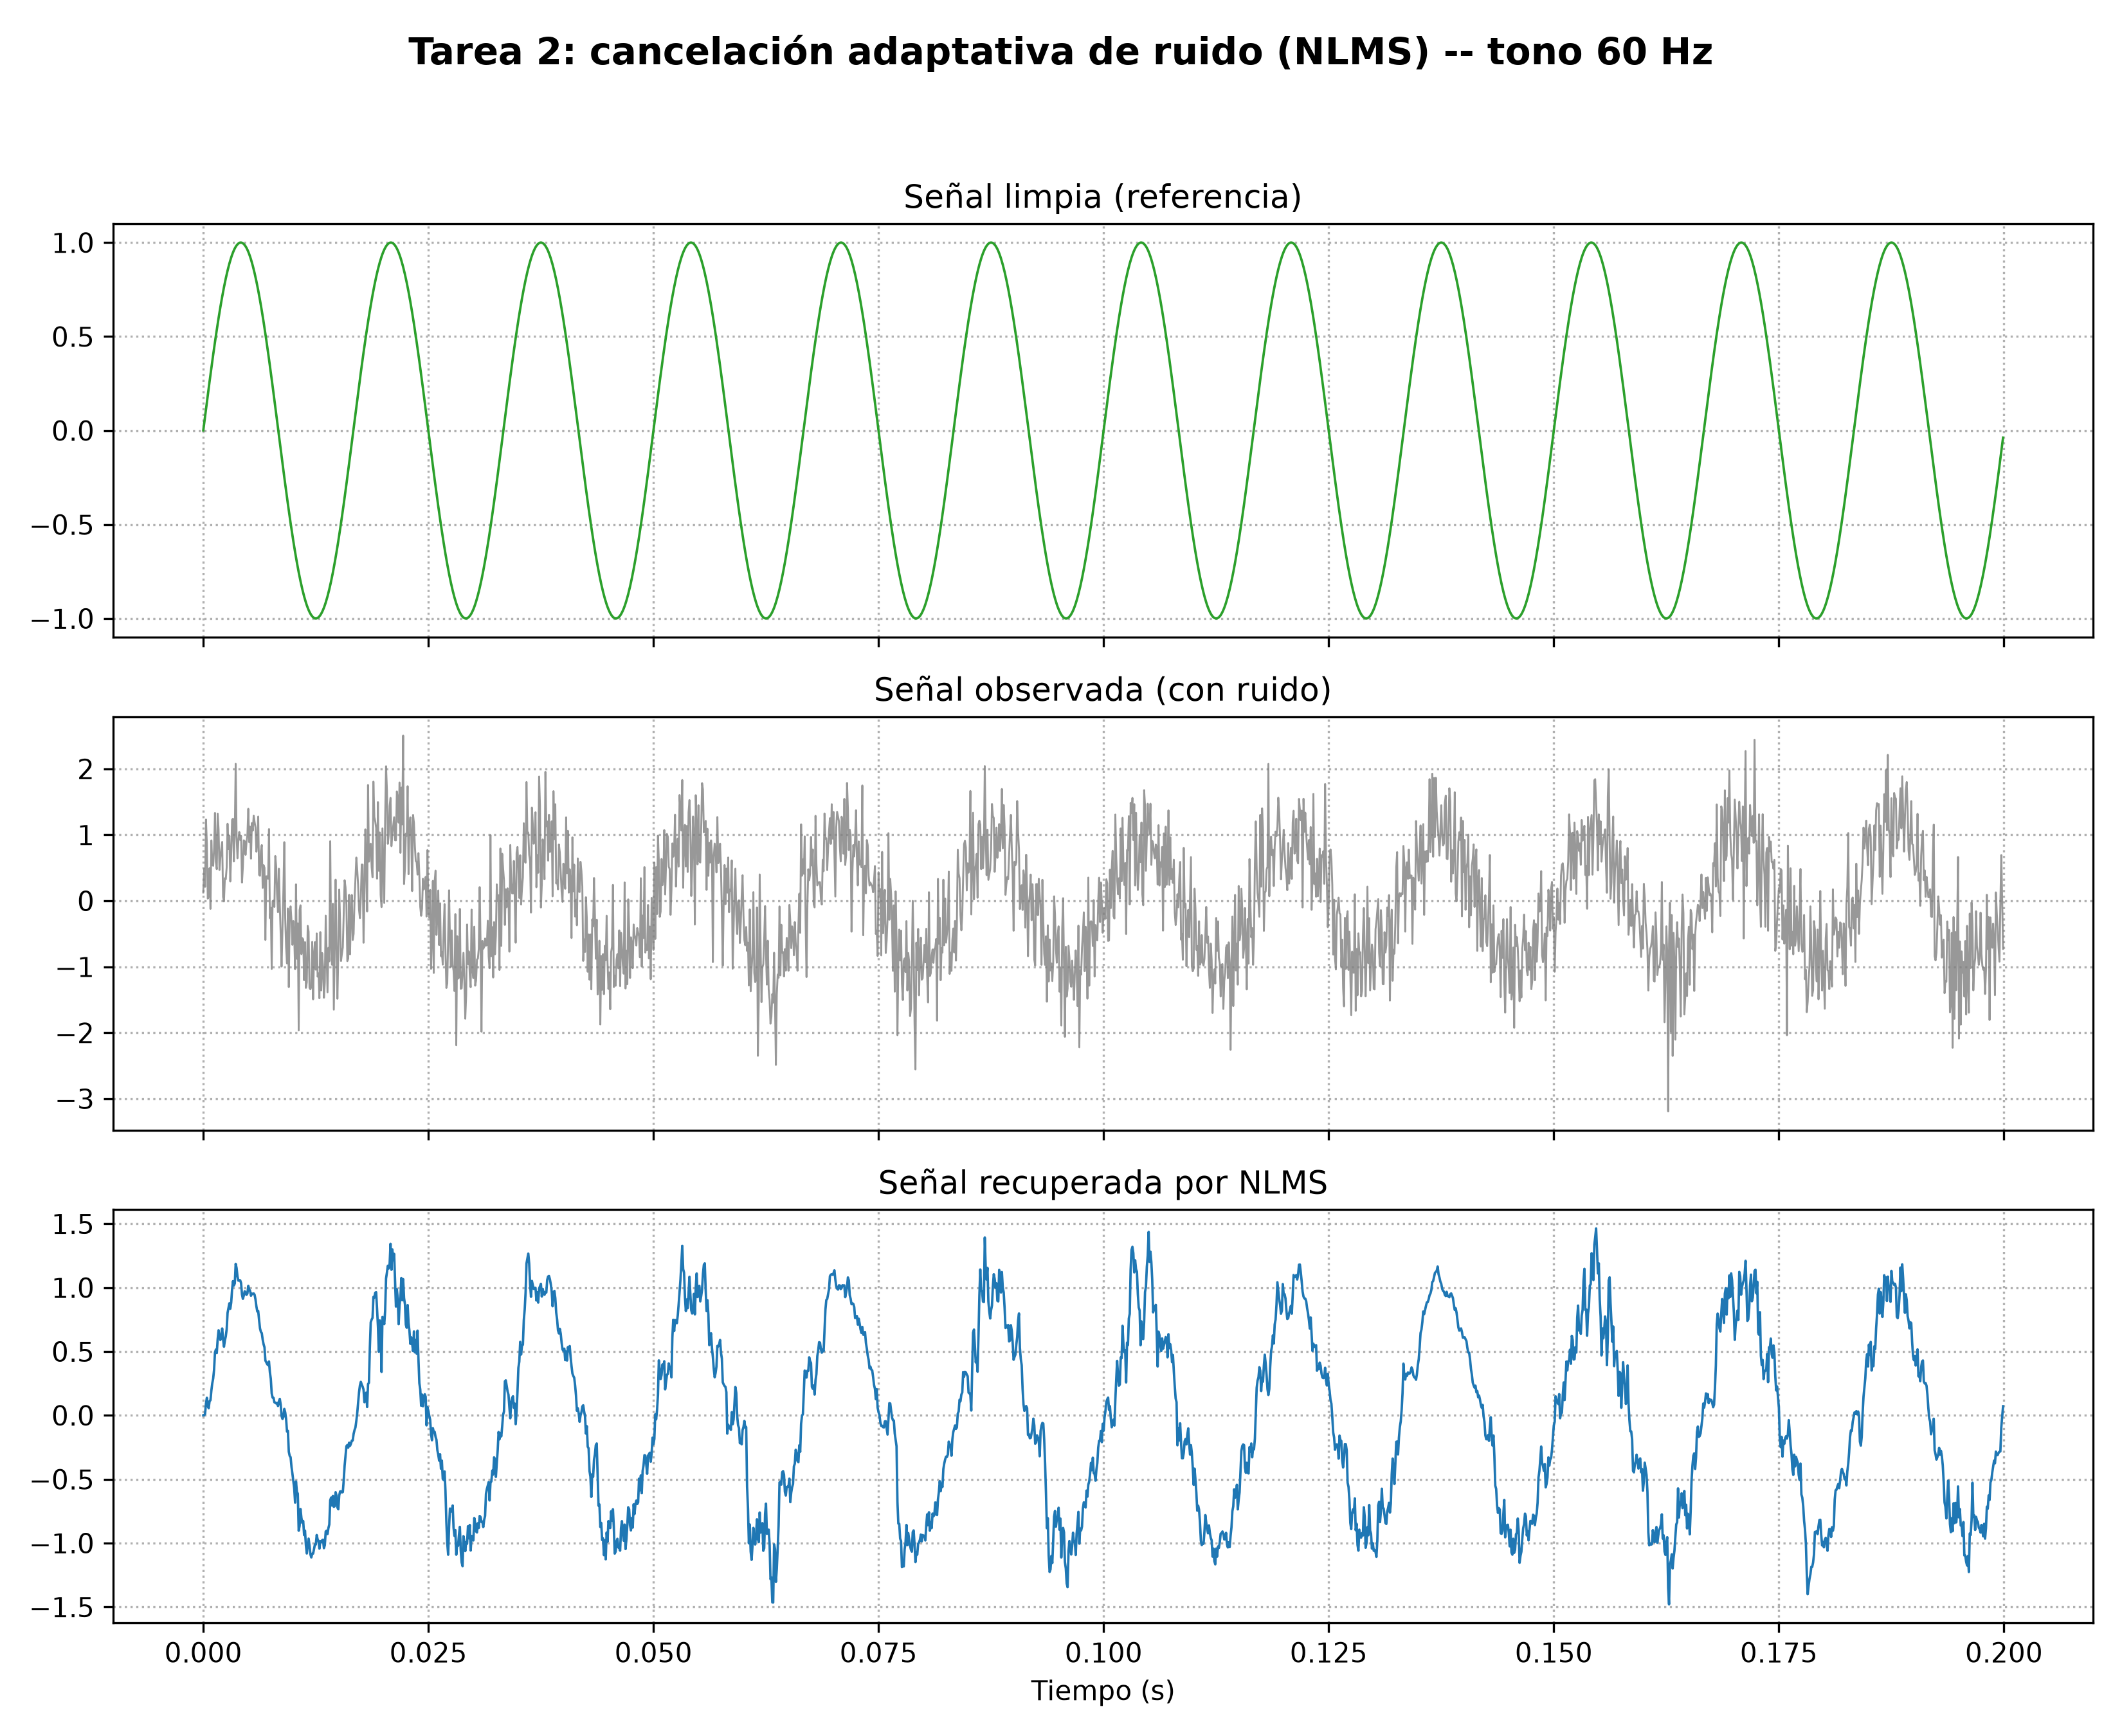
\includegraphics[width=\columnwidth]{work_twelve_t2_noise_cancellation_tone.png}
\caption{NLMS: cancelación adaptativa de ruido sobre un tono de 60~Hz.}
\label{fig:work_twelve_t2a}
\end{figure}

\begin{figure}[!t]
\centering
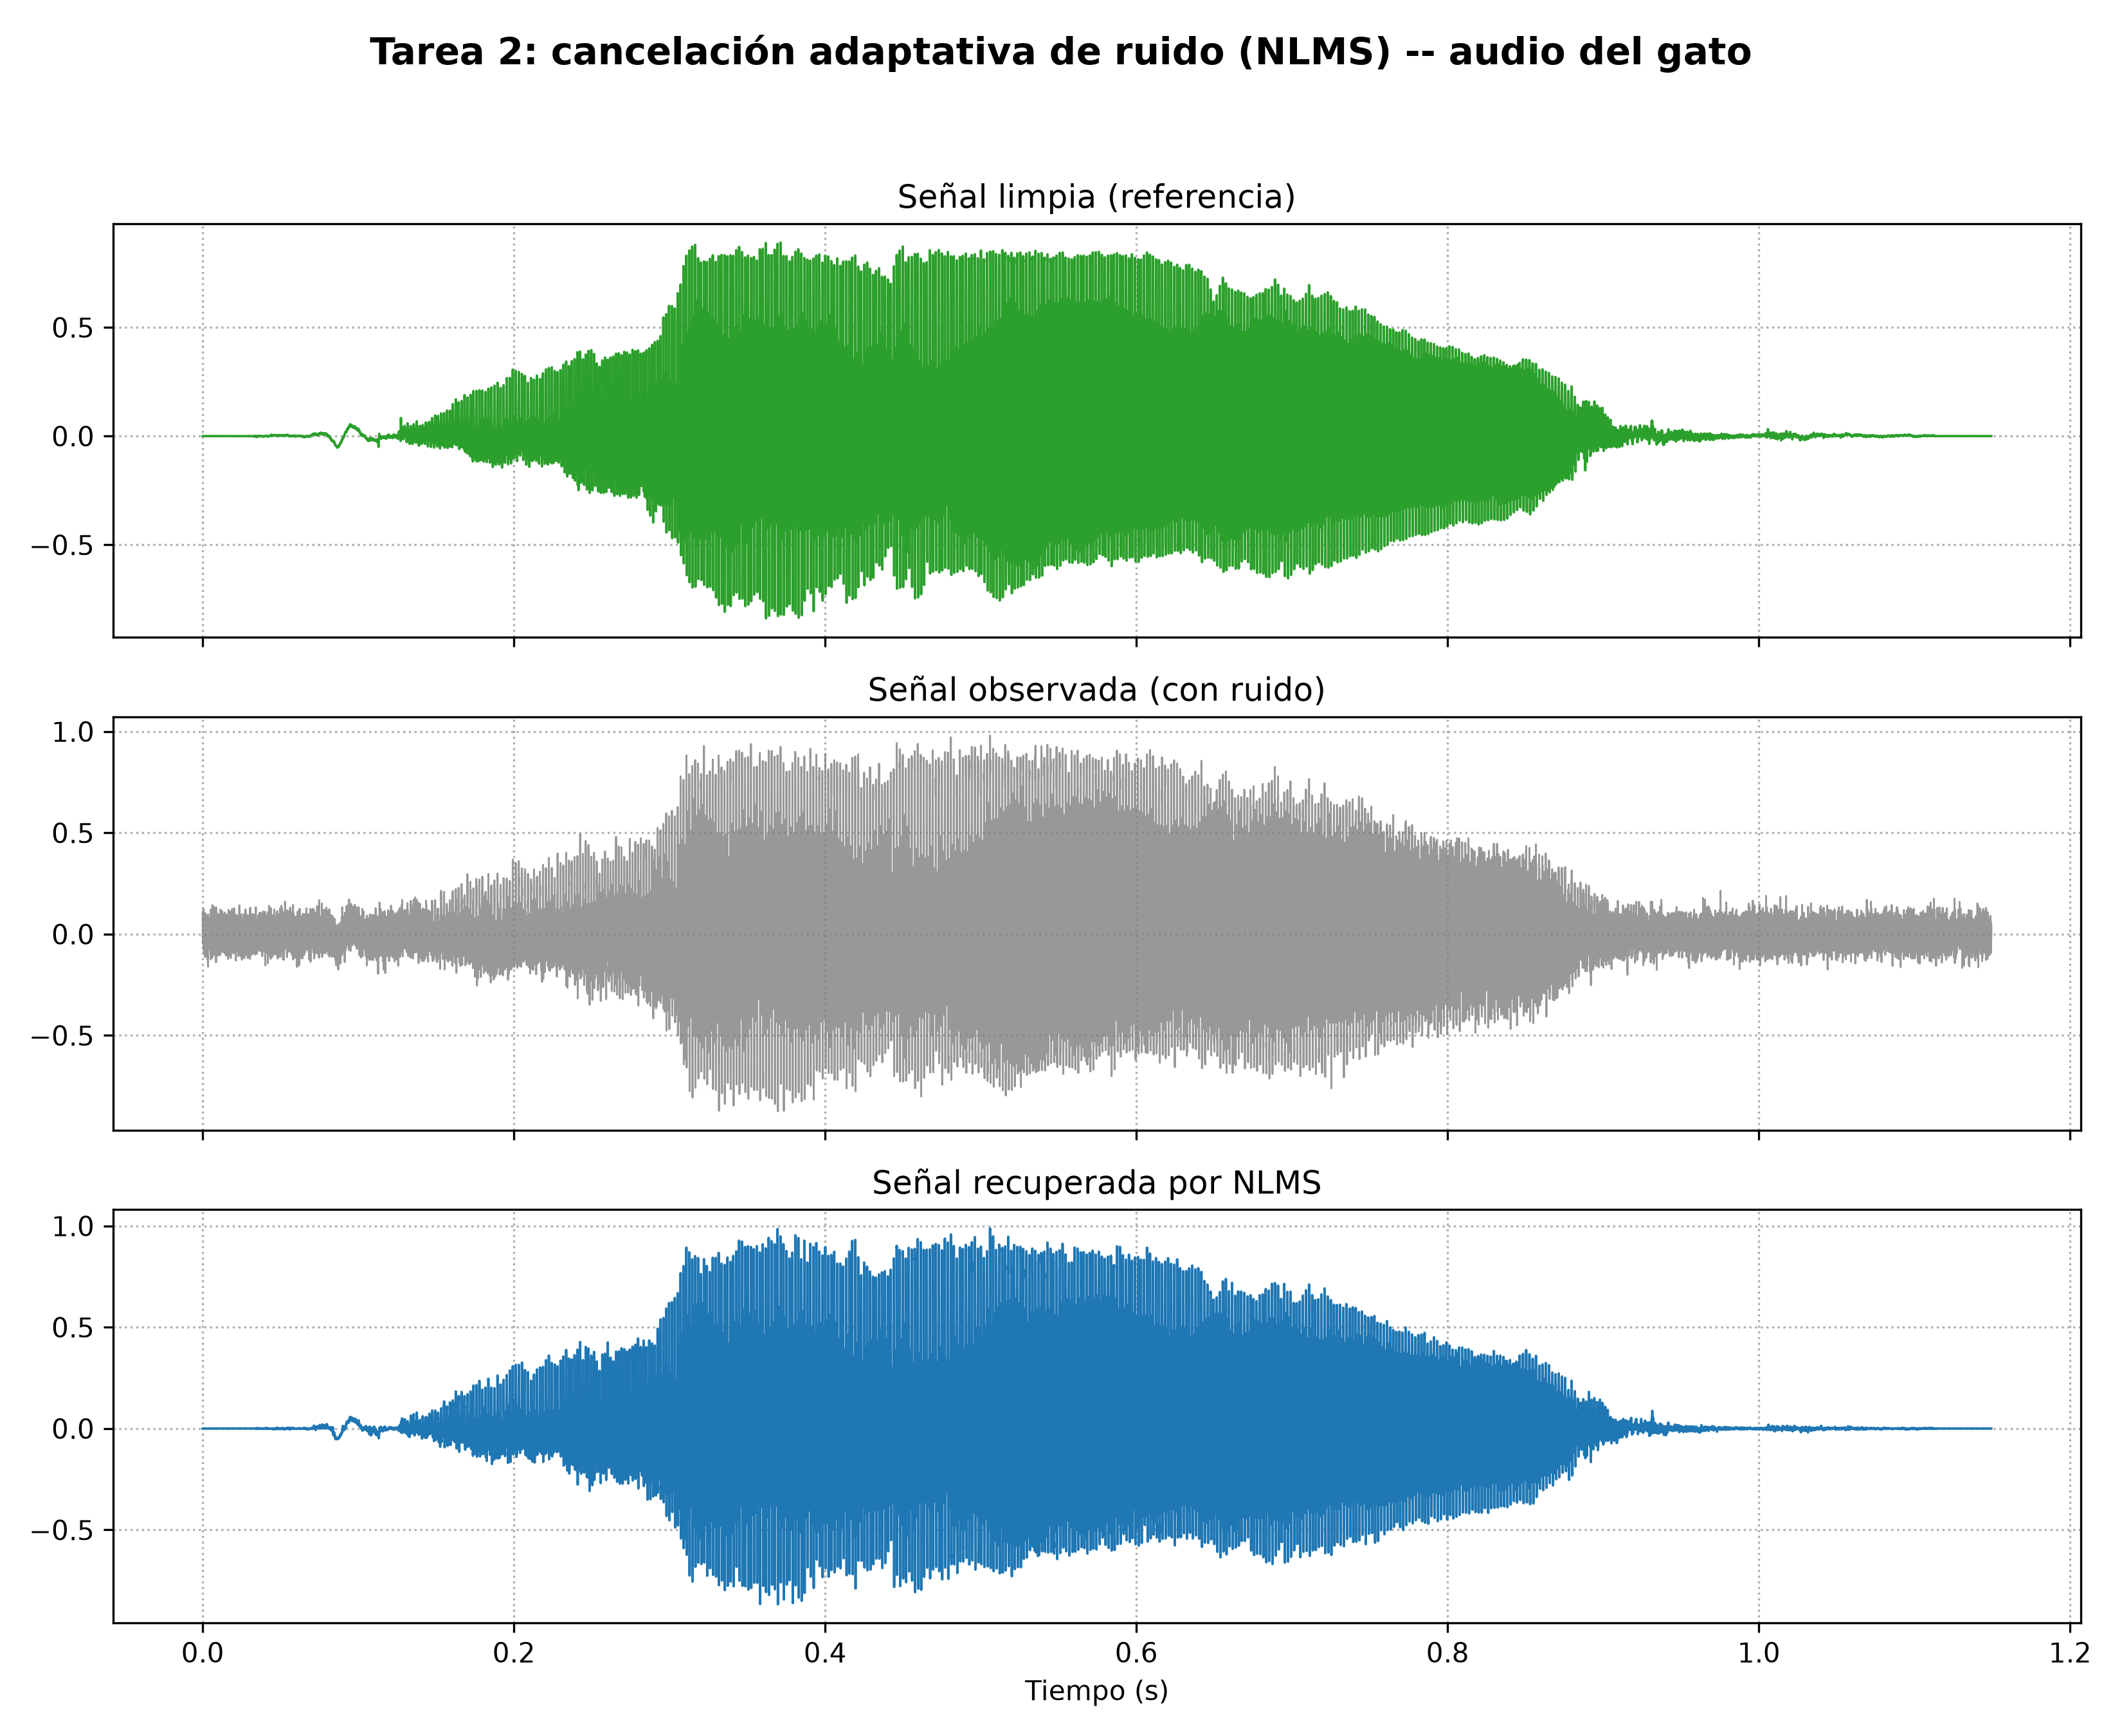
\includegraphics[width=\columnwidth]{work_twelve_t2_noise_cancellation_cat.png}
\caption{NLMS: cancelación adaptativa de ruido sobre una grabación de audio real.}
\label{fig:work_twelve_t2b}
\end{figure}

\subsubsection{NLMS frente a LMS bajo potencia de entrada no estacionaria}
\label{sec:nlms_vs_lms}

El experimento más relevante de este trabajo busca exponer, de forma
cuantitativa y no solo cualitativa, la ventaja práctica que justifica
preferir NLMS sobre LMS en aplicaciones reales. Para ello se repitió el
problema de identificación de sistema con una señal de entrada cuya
amplitud cambia abruptamente por un factor de 40 a la mitad del
experimento —simulando, de forma simplificada, el tipo de variación de
potencia que aparece en señales de voz (pasajes hablados frente a
silencios) o en canales de comunicación con desvanecimiento. Se
comparó NLMS contra una reimplementación local de LMS con un único
valor de $\mu$, fijo durante todo el experimento y elegido
deliberadamente para que el filtro se mantenga estable durante el
segmento de \emph{mayor} potencia —la elección natural que haría un
diseñador que solo puede fijar un parámetro antes de observar cómo se
comportará la señal en el tiempo.

Los resultados (Fig.~\ref{fig:work_twelve_t3}) muestran una diferencia
sustancial: en el segmento de \emph{menor} potencia, el error cuadrático
medio en estado estacionario de LMS fue de 0.03967, frente a 0.00117
para NLMS —es decir, LMS mantiene un error aproximadamente 34 veces
mayor que NLMS bajo las mismas condiciones de entrada y el mismo
sistema desconocido a identificar. La razón es exactamente la prevista
por la teoría: el $\mu$ de LMS, al estar fijado por la necesidad de
permanecer estable en el segmento de alta potencia, resulta demasiado
pequeño para converger con la misma eficacia cuando la señal de entrada
se debilita; NLMS, en cambio, al normalizar su paso por la energía
instantánea de la entrada, incrementa automáticamente su paso efectivo
en el segmento de baja potencia sin arriesgar la estabilidad en el
segmento de alta potencia, porque en ese segmento el denominador de
normalización crece en la misma proporción.

Esta observación no es un detalle menor de implementación: es la razón
estructural por la cual NLMS, y no LMS, es la variante preferida en la
inmensa mayoría de aplicaciones prácticas de filtrado adaptativo sobre
señales de audio y voz —precisamente el tipo de señal cuya potencia
varía de forma natural y constante en el tiempo— incluyendo
cancelación de eco acústico en telefonía y ecualización adaptativa de
canales de comunicación.

\begin{figure}[!t]
\centering
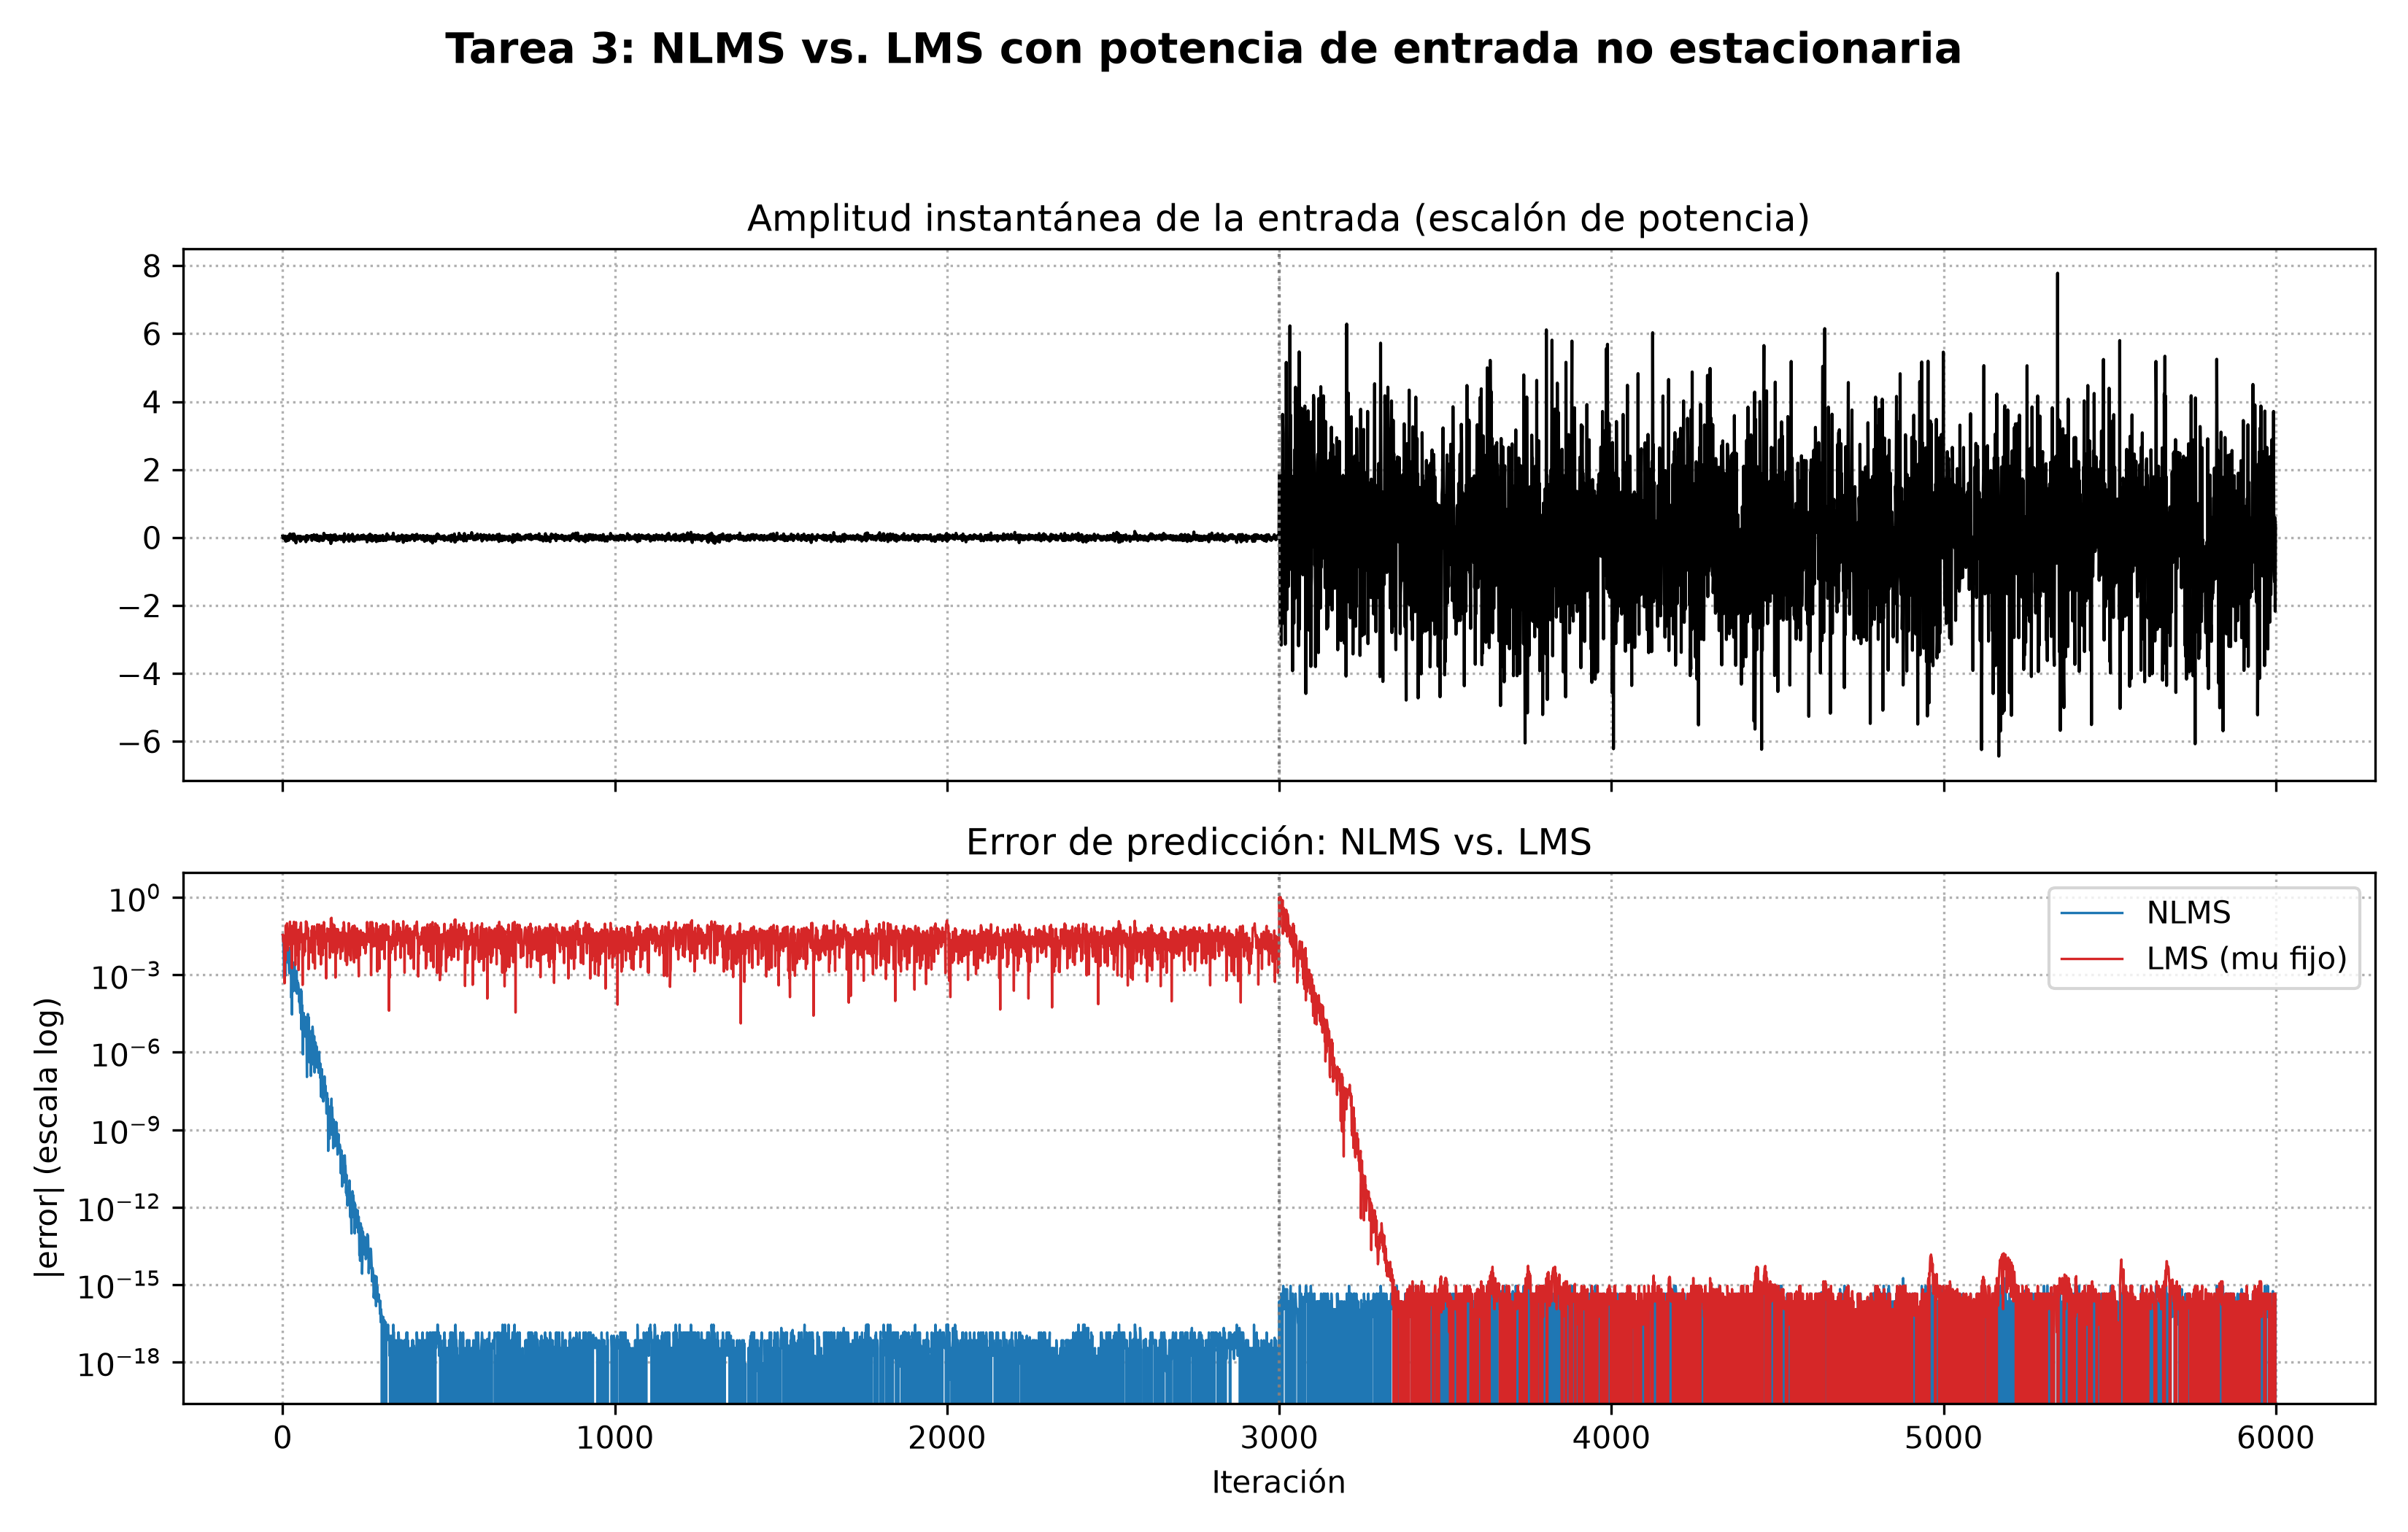
\includegraphics[width=\columnwidth]{work_twelve_t3_nlms_vs_lms_varying_power.png}
\caption{Comparación NLMS vs.\ LMS sobre una entrada con un cambio abrupto de potencia (factor 40) a mitad del experimento. El panel muestra el error de identificación de cada algoritmo en ambos segmentos, evidenciando que NLMS mantiene un error bajo y consistente en ambos mientras que LMS, con un $\mu$ fijo conservador, degrada su desempeño en el segmento de menor potencia.}
\label{fig:work_twelve_t3}
\end{figure}


\section{Conclusiones}
\label{sec:conclusiones}

Los dos filtros adaptativos implementados desde cero en este informe
—LMS en WORK\_ELEVEN y NLMS en WORK\_TWELVE— lograron identificar
ciegamente un sistema FIR desconocido a partir únicamente de pares
entrada/salida, recuperando sus coeficientes reales con un error
prácticamente nulo, y cancelar ruido correlacionado tanto sobre una
señal sintética de banda angosta como sobre una grabación de audio
real de contenido espectral más complejo. Estos resultados confirman
experimentalmente, con implementaciones propias y auditables, que el
mecanismo de descenso de gradiente estocástico subyacente a ambos
algoritmos converge de forma robusta en problemas representativos de
identificación de sistemas y cancelación de ruido, sin depender de una
función de filtrado adaptativo ya empaquetada por una librería externa
cuyo funcionamiento interno permanecería opaco.

El análisis de convergencia de LMS frente al tamaño de paso $\mu$
confirmó de forma cuantitativa la cota teórica de estabilidad
$\mu < 2/\lambda_{\max}$: la convergencia observada fue lenta para
$\mu$ muy por debajo de esa cota, rápida y estable para valores
intermedios, y francamente divergente para un $\mu$ ligeramente por
encima del límite teórico calculado para esta configuración
experimental ($\approx 0.4$). Este resultado es relevante más allá de
su valor demostrativo inmediato: evidencia que la elección del tamaño
de paso en un sistema LMS real no puede hacerse de forma arbitraria o
puramente empírica, sino que debe fundamentarse en una estimación,
aunque sea aproximada, de la potencia de la señal de entrada y del
número de coeficientes del filtro.

La comparación directa entre NLMS y LMS bajo una señal de entrada con
potencia no estacionaria constituye el resultado más significativo de
este informe desde el punto de vista práctico: bajo las mismas
condiciones de entrada y el mismo sistema desconocido, LMS con un
$\mu$ fijo —elegido para ser estable en el segmento de mayor
potencia— exhibió un error de identificación aproximadamente 34 veces
mayor que NLMS en el segmento de menor potencia. Esta diferencia no es
un artefacto de la elección particular de parámetros del experimento,
sino la consecuencia directa y esperada de la normalización por
energía instantánea que define a NLMS, y constituye la razón
estructural —no meramente una preferencia de implementación— por la
cual NLMS es el algoritmo de elección en la inmensa mayoría de
aplicaciones reales de filtrado adaptativo sobre señales no
estacionarias en potencia, como la voz humana o los canales de
comunicación con desvanecimiento.

Como trabajo futuro, resultaría natural extender ambos laboratorios
con una variante de paso variable adicional, como LMS normalizado con
factor de olvido (\textit{leaky NLMS}) para mejorar la robustez frente
a sistemas desconocidos que cambian lentamente en el tiempo, o con
RLS (\textit{Recursive Least Squares}) como punto de comparación de
convergencia mucho más rápida a costa de un mayor costo computacional
por iteración —un compromiso distinto al explorado aquí, pero
igualmente relevante en la práctica del procesamiento adaptativo de
señales.

\begin{thebibliography}{00}

\bibitem{widrowhoff} B. Widrow, M. E. Hoff, ``Adaptive switching
circuits,'' \textit{IRE WESCON Convention Record}, 1960, pp. 96-104.

\bibitem{haykin} S. Haykin, \textit{Adaptive Filter Theory}, 5th ed.,
Pearson, 2014.

\bibitem{sayed} A. H. Sayed, \textit{Adaptive Filters}, Wiley-IEEE
Press, 2008.

\bibitem{scipy} The SciPy community, ``SciPy Reference Guide,'' [En
línea]. Disponible: \url{https://docs.scipy.org/}.

\end{thebibliography}


\end{document}
